\documentclass[journal,brazil,english]{IEEEtran}

\usepackage[pdftex]{graphicx}
\graphicspath{{../pdf/}{../jpeg/}}
\DeclareGraphicsExtensions{.pdf,.jpeg,.png}
\usepackage[brazil]{babel}
\usepackage[utf8]{inputenc}
\usepackage[T1]{fontenc}
\usepackage[cmex10]{amsmath}
\usepackage{amssymb}
\usepackage{mathabx}
\usepackage{algorithmic}
\usepackage{array}
\usepackage{float}
\usepackage{mdwmath}
\usepackage{mdwtab}
\usepackage{eqparbox}
\usepackage{url}
\usepackage{caption}
\usepackage{multicol}
%\newtheorem{theorem}{\textbf{Teorema}}
%\newtheorem{definition}{\textbf{Definição}}

\hyphenation{op-tical net-works semi-conduc-tor}

\begin{document}
\title{Projeto de Controladores por Alocação de Polos Aplicados a um Sistema de Suspensão Ativa}

\author{Joacy Mesquita da Silva, Márcia Lissandra Machado Prado}

\maketitle

\begin{abstract}
This work presents the design of controllers by pole placement for an active suspension system developed by Quanser. The project can be divided into system modeling, design of the controllers, and analysis of the obtained results. The intention is to ensure that the system meets the requirements of the project, and also remains stable.
\end{abstract}

\begin{IEEEkeywords}
Control Theory, Pole Placement, Active Suspension System.
\end{IEEEkeywords}

\selectlanguage{brazil}
\begin{abstract}
Esse trabalho apresenta o projeto de controladores por Alocação de Polos para um sistema de suspensão ativa desenvolvido pela Quanser. O projeto pode ser dividido em modelagem do sistema, projeto dos controladores, e a análise dos resultados obtidos. A intenção é garantir que o sistema atenda aos requisitos do projeto, e também permaneça estável.
\end{abstract}

\begin{IEEEkeywords}
Teoria de Controle, Alocação de Polos, Sistema de Suspensão Ativa.
\end{IEEEkeywords}

\IEEEpeerreviewmaketitle

\section{Introdução}\label{introducao}
Os sistemas de controle são importantes em diversos campos da engenharia e da ciência. Eles são utilizados nas mais diversas áreas da indústria \cite{ogata}. Em veículos espaciais, sistemas robóticos, e operações industriais que envolvam o controle de temperatura, vazão, pressão, estabilização, direção, estão exemplos de sua utilização \cite{nise}.

%A Teoria de Controle Robusto estuda métodos para a construção de controladores com o propósito de melhorar significativamente o desempenho de sistemas de controle complexos, aplicáveis especialmente à indústria \cite{almeida}. Quando, no projeto do controlador, há o desejo de especular a existência de erros ou incertezas entre a planta real e o seu modelo matemático, tal teoria é empregada \cite{ogata}.

Na literatura de controle não se encontra com facilidade o projeto de controladores por função de transferência. O problema compreende o encontro de um polinômio característico, resultante de uma alocação de polos, que atenda às especificações do projeto \cite{lordelo}.

O problema de projeto de controladores por realimentação de estados para sistemas lineares invariantes no tempo tem sido extensamente tratado na literatura de controle \cite{ogata, nise, dorf}. Quando se refere à alocação de polos, o problema consiste em assinalar um ganho de realimentação de estados capaz de alocar todos os polos do sistema em malha fechada nas posições desejadas \cite{ogata}.

O Sistema de Suspensão Ativa é um exemplo de sistema mecânico empregado em automóveis e em aplicações industriais. As suspensões veiculares têm por finalidade suportar de forma adequada o chassi do veículo, fazendo isolamento das vibrações causadas por irregularidades do terreno; manter o contato dos pneus com o solo de modo a manter o carro o mais estável possível; e proporcionar melhor dirigibilidade e conforto aos seus ocupantes \cite{corte-real}.

O desenvolvimento de um controlador para sistemas de suspensão ativa apresenta relevância, pelo fato desses sistemas possuírem função importante na indústria automobilística e em diversas aplicações industriais.

Este trabalho tem por objetivo realizar o projeto de controladores por alocação de polos utilizando função de transferência, e por realimentação de estados, a serem aplicados ao sistema de suspensão ativa.

O trabalho está dividido da seguinte forma, na Seção \ref{fundamentacao} são apresentados conceitos de teoria de controle, alocação de polos, sistemas de controle no espaço de estados; nas Seções \ref{funcaotransferencia} e \ref{projetoespacoestados} são exibidas as metodologias utilizadas para os projetos dos controladores, representando o sistema como função de tranferência e como espaço de estados, respectivamente; na Seção \ref{resultados} são expostos e analisados os resultados obtidos com os controladores projetados; e na Seção \ref{conclusao} são relatadas as conclusões obtidas.

\section{Fundamentação Teórica}\label{fundamentacao}
Nesta Seção são apresentados os conceitos teóricos que fundamentam o trabalho. São abordados conceitos de teoria de controle, alocação de polos em função de transferência, sistemas no espaço de estados, e alocação de polos em espaço de estados.

\subsection{Teoria de Controle}
É possível descrever os sistemas físicos, sejam eles mecânicos, hidráulicos ou elétricos, através da modelagem matemática utilizando as leis da física, normalmente utiliza-se a representação por equações diferenciais ordinárias \cite{dorf}. A análise no domínio do tempo desses sistemas de equações diferenciais é a base da teoria de controle \cite{ogata}.

Uma maneira de proporcionar a simplificação dos cálculos necessários para essa análise é a utilização da transformada de Laplace. Nesse caso o sistema passa a ser descrito por sua função de transferência, que é a relação entre a transformada de Laplace do sinal de saída e a transformada de Laplace do sinal de entrada. Conhecer a natureza e obter uma descrição completa sobre a dinâmica de um sistema de controle pode ser possível através da função de transferência do mesmo \cite{ogata}. Um exemplo de função de transferência pode ser encontrado na Equação (\ref{tf}).

\begin{equation}\label{tf}
G(s) = \frac{Y(s)}{X(s)} = \frac{b_{0}s^m + b_{1}s^{m-1} + \cdots + b_{m-1}s + b_m}{a_{0}s^n + a_{1}s^{n-1} + \cdots + a_{n-1}s + a_n}
\end{equation}

Onde $n$ e $m$ são inteiros e $n$ representa a ordem do sistema. A saída do sistema é $Y(s)$, e a entrada é $X(s)$, os $a$'s e os $b$'s são coeficientes e $s$ uma variável complexa.  Os zeros são as raízes do polinômio do numerador da função de transferência, enquanto os polos são as raízes do polinômio do denominador da função de transferência.

\subsubsection{Realimentação}
Em um sistema de controle, a realimentação ocorre quando se utiliza o sinal de saída do sistema para compará-lo com o sinal de referência. Tendo conhecimento da resposta desejada para um sistema de controle, pode ser gerado um sinal proporcional ao erro entre a resposta desejada e a resposta real. O controle da planta (sistema a ser controlado) pode ser realizado através da utilização desse sinal, resultando em uma sequência de operações em malha fechada chamada de sistema com realimentação \cite{dorf}.

O sistema é denomidado sistema de malha aberta quando não possui realimentação. Nesse caso, um sinal de saída é gerado diretamente pela interação do sinal de entrada e o sistema \cite{franklin}.

Nos sistemas de malha aberta, o sinal de saída não exerce ação de controle sobre o sistema, ele não é medido nem comparado com o sinal de entrada de referência. Por isso, uma condição fixa de operação existe para cada entrada de referência nos sistemas de malha aberta. A precisão do sistema está relacionada a uma calibração. De forma prática, os sistemas de controle em malha aberta  só podem ser utilizados quando se conhece a relação entre a entrada e a saída, além de não haver distúrbios internos ou externos \cite{ogata}.

Já nos sistemas de controle de malha fechada, o sinal de saída exerce uma ação de controle sobre o sistema. O sinal de erro, que é a diferença entre o sinal de entrada e o de saída, realimenta o sistema de modo a diminuir o erro e levar a saída para o valor desejado \cite{ogata}.

A Figura \ref{malhaaberta} ilustra o diagrama de blocos de um sistema em malha aberta, enquanto a Figura \ref{malhafechada} ilustra o diagrama de blocos de um sistema em malha fechada.
 
\begin{figure}[H]
	\centering
	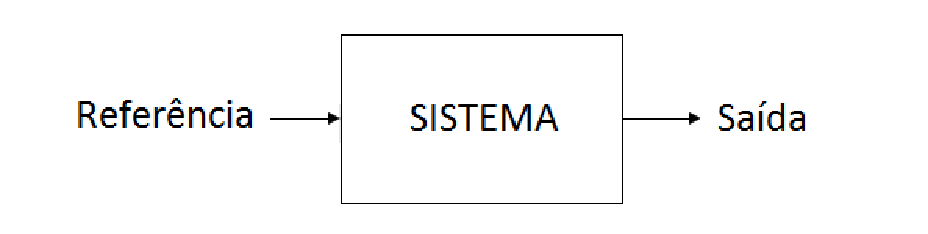
\includegraphics[width=\columnwidth]{./imagens/malha_aberta.pdf}
    \renewcommand{\figurename}{Fig.}
    \caption{Diagrama de Sistema em Malha Aberta.}
	\label{malhaaberta}
\end{figure}

\begin{figure}[H]
	\centering
	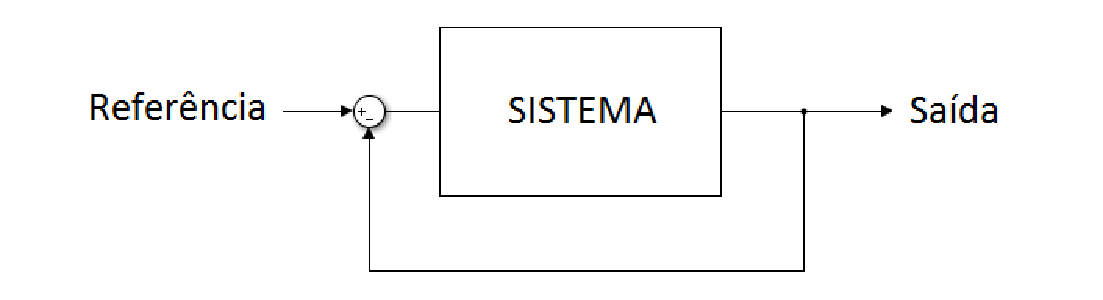
\includegraphics[width=\columnwidth]{./imagens/malha_fechada.pdf}
    \renewcommand{\figurename}{Fig.}
    \caption{Diagrama de Sistema em Malha Fechada.}
	\label{malhafechada}
\end{figure}

\subsubsection{Estabilidade}
No projeto de sistemas de controle, a estabilidade é um objetivo importantíssimo. Um sistema de controle de malha fechada que não apresenta estabilidade geralmente não tem nenhuma aplicação real, por conta disso procura-se utilizar procedimentos e ferramentas que proporcionem o projeto de sistemas estáveis \cite{dorf}.

A estabilidade de um sistema é determinada através da localização dos seus polos de malha fechada no plano $s$. É estável todo sistema onde todos os polos estiverem localizados no semiplano esquerdo do plano $s$. Se qualquer um dos polos estiver situado  no semiplano direito do plano $s$ o sistema é instável \cite{ogata}.

Em um diagrama de polos e zeros, de forma padrão, os polos do sistema são representados por `X', e os zeros são representados por `O'.

A Figura \ref{estavel} apresenta o diagrama de polos e zeros de um sistema estável, com polos localizados em $s=-25$, $s=-10$ e $s=-5$. A Figura \ref{instavel} apresenta o diagrama de polos e zeros de um sistema instável, com polos localizados em $s=-25$, $s=-10$ e $s=5$.

\begin{figure}[H]
	\centering
	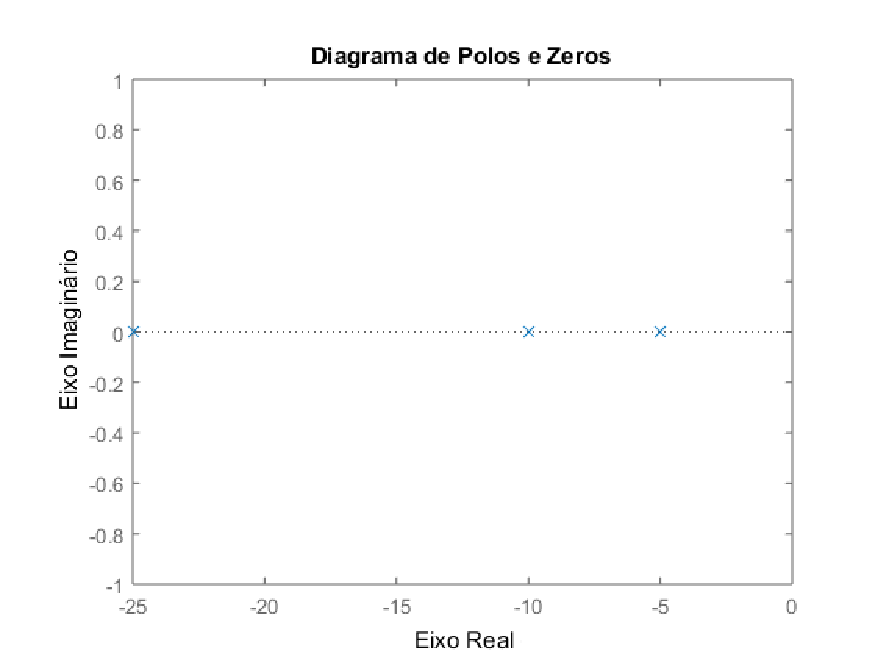
\includegraphics[width=\columnwidth]{./imagens/sistema_estavel.pdf}
    \renewcommand{\figurename}{Fig.}
    \caption{Diagrama de Polos e Zeros de um Sistema Estável.}
	\label{estavel}
\end{figure}

\begin{figure}[H]
	\centering
	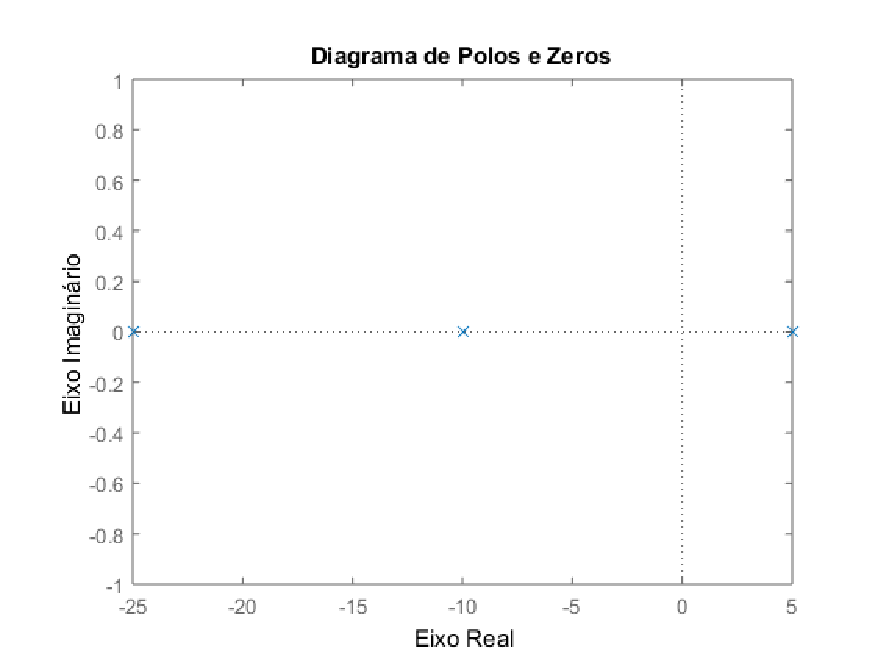
\includegraphics[width=\columnwidth]{./imagens/sistema_instavel.pdf}
    \renewcommand{\figurename}{Fig.}
    \caption{Diagrama de Polos e Zeros de um Sistema Instável.}
	\label{instavel}
\end{figure}

\subsection{Alocação de Polos em Função de Transferência}\label{alocacaoFT}
A técnica de controle por Alocação de Polos parte da suposição de que estabilidade e várias especificações de desempenho podem ser atingidas com a utilização da realimentação dinâmica da saída para alocar os polos de malha fechada do sistema em posições apropriadas do plano complexo $s$ \cite{maitelli}.

Dentre vários tipos de estruturas de sistemas de controle \cite{ogata}, considere o sistema de controle contínuo com realimentação unitária, linear e invariante no tempo, com uma entrada e uma saída (SISO), representado na Figura \ref{ggc}.

\begin{figure}[H]
	\centering
	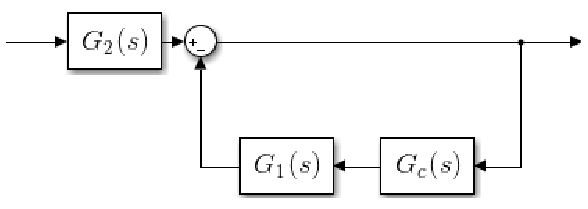
\includegraphics[width=\columnwidth]{./imagens/siso.pdf}
    \renewcommand{\figurename}{Fig.}
    \caption{Sistema SISO com realimentação.}
	\label{ggc}
\end{figure}

A função $G_1(s)$, de ordem $m$, é a função de transferência da saída em relação a força de controle. A função $G_2(s)$, de ordem $n$, é a função de transferência da saída em relação a uma perturbação do sistema. E a função $G_c(s)$, de ordem $r$, é a função de transferência de um controlador a ser aplicado a $G_1(s)$. As funções $G_1(s)$, $G_2(s)$ e $G_c(s)$ podem ser escritas no formato

$G_1(s) := \frac{nG_1(s)}{dG_1(s)}$, $G_2(s) := \frac{nG_2(s)}{dG_2(s)}$ e $G_c(s) := \frac{nG_c(s)}{dG_c(s)}$,
onde
\begin{equation}\label{nG1}
nG_1(s) := a_1s^m + a_2s^{m-1} + \cdots + a_{m+1},
\end{equation}
\begin{equation}\label{dG1}
dG_1(s) := a_{m+2}s^m + a_{m+3}s^{m-1} + \cdots + a_{2m+2},
\end{equation}
\begin{equation}\label{nG2}
nG_2(s) := c_1s^n + c_2s^{n-1} + \cdots + c_{n+1},
\end{equation}
\begin{equation}\label{dG2}
dG_2(s) := c_{n+2}s^n + c_{n+3}s^{n-1} + \cdots + c_{2n+2},
\end{equation}
\begin{equation}\label{nGc}
nG_c(s) := w_1s^r + w_2s^{r-1} + \cdots + w_{r+1},
\end{equation}
\begin{equation}\label{dGc}
dG_c(s) := w_{r+2}s^r + w_{r+3}s^{r-1} + \cdots + w_{2r+2}.
\end{equation}
com $a_{m+2} \neq 0$ e $c_{n+2} \neq 0$.

Inicialmente, assume-se que os coeficientes da planta $(a_1, a_2, \ldots, a_{2m+2})$, e $(c_1, c_2, \ldots, c_{2n+2})$ são precisamente conhecidos. Os parâmetros de projeto do controlador $(w_1, w_2, \ldots, w_{2r+2})$ devem ser selecionados de maneira que as especificações de desempenho, traduzidas em localizações dos polos do sistema em malha fechada, sejam satisfeitas com um controlador de menor ordem possível para que o sistema resultante, em malha fechada, tenha um conjunto de $m+n+r$ polos desejados \cite{maitelli}. O sistema em malha fechada é representado por

\begin{equation}\label{ts}
T(s) = G_2(s)\frac{1}{1+G_1(s)G_c(s)}
\end{equation}

\begin{equation}\label{ts1}
T(s) = \frac{nG_2(s)}{dG_2 (s)}\frac{1}{\frac{dG_1(s)dG_c(s)+nG_1(s)nG_c(s)}{dG_1(s)dG_c(s)}}
\end{equation}

\begin{equation}\label{ts2}
T(s) = \frac{nG_2(s)dG_1(s)dG_c(s)}{dT(s)}
\end{equation}
com $dT(s) = dG_2(s)dG_1(s)dG_c(s)+dG_2(s)nG_1(s)nG_c(s)$.

A técnica tem por objetivo alocar os polos de $T(s)$, ou seja, as raízes de $dT(s)$. Pela Equação (\ref{ts2}) pode ser visto que novos zeros, raízes de $nT(s)$, são introduzidos na função de transferência de malha fechada, os polos de $T(s)$ são resultados dos deslocamentos dos polos de $G_1(s)$, $G_2(s)$ e de $G_c(s)$. Para que os coeficientes das funções de transferência sejam reais, os polos complexos conjugados devem ser alocados aos pares \cite{maitelli}.

Nesse contexto, o problema de alocação de polos é resumido na solução da equação abaixo, referente ao denominador do sistema em malha fechada

\begin{equation}\label{diof}
\begin{matrix}
dT(s) = dG_2(s)dG_1(s)dG_c(s)+\\dG_2(s)nG_1(s)nG_c(s)
\end{matrix}
\end{equation}
reescrevendo $dT(s)$ em função de seus coeficientes, temos:

\begin{equation}
dT(s) := b_1 s^{m+n+r} + b_2 s^{m+n+r-1} + \cdots + b_{m+n+r+1}
\end{equation}

Contudo, em vez de resolver a Equação (\ref{diof}) de forma direta, pode-se transformá-la em um sistema de equações algébricas lineares. Com isso, substituindo todos os polinômios em (\ref{diof}) e associando os coeficientes com as potências semelhantes em $s$, obtém-se um sistema de $m+n+r+1$ equações lineares da forma

\begin{center}
$a_1 c_{n+2} w_1 + a_{m+2} c_{n+2} w_{r+2} = b_1$,
$a_2 c_{n+2} w_1 + a_1 c_{n+2} w_2 + \cdots + a_{m+3} c_{n+2} w_{r+2} + a_{m+2} c_{n+2} w_{r+3} = b_2$,

$\vdots$

$a_{m+1} c_{2n+2} w_{r+1} + a_{2m+2} c_{2n+2} w_{2r+2} = b_{m+n+r+1}$.
\end{center}

Por conveniência, define-se $p := m+ n + r + 1$ e
$q := 2r + 2$. A Equação (\ref{diof}) pode ser escrita como uma equação linear no formato
\begin{equation}\label{silvester}
Aw=b,
\end{equation}
na qual $A$ é a matriz formada pelos coeficientes de $nG_1(s)$ e $dG_1(s)$, multiplicados pelos coeficientes de $dG_2(s)$, $w$ é o vetor composto pelos coeficientes de $G_c(s)$, e $b$ é o vetor constituído pelos coeficientes de $dT(s)$.

Sendo  $A \in \mathbb{R}^{p \times q}$,
\begin{equation}
w:=\begin{bmatrix}
w_1 &
w_2 &
\ldots &
w_q
\end{bmatrix}^T \in \mathbb{R}^q
\end{equation}
e
\begin{equation}
b:=\begin{bmatrix}
b_1 &
b_2 &
\ldots &
b_p
\end{bmatrix}^T \in \mathbb{R}^p.
\end{equation}

Na Equação (\ref{silvester}), a matriz $A$ é a matriz de Sylvester \cite{maitelli} referente às funções $G_1(s)$ e $G_2(s)$. Os coeficientes de $nG_1(s)$, em ordem decrescente de potências de $s$, multiplicados pelos coeficientes de $dG_2(s)$, compõem a primeira coluna de $A$. A primeira coluna deslocada uma posição para baixo forma a segunda coluna, o mesmo acontece de forma sucessiva para as $r+1$ primeiras colunas de $A$. Para formar a $(r + 2)$-ésima coluna de $A$ em diante, se repete o procedimento anterior, mais os coeficientes de $dG_1(s)$ multiplicados pelos coeficientes de $dG_2(s)$ compõem estas colunas \cite{maitelli}.

\subsection{Sistemas de Controle no Espaço de Estados}\label{espacoestados}

O estado de um sistema dinâmico pode ser definido como o menor conjunto de variáveis de estado de modo que o conhecimento destas variáveis no instante $t=t_0$, e da entrada para $t\geqslant t_0$, determina completamente o comportamento do sistema para qualquer instante $t \geqslant t_0$ \cite{ogata}.

As  variáveis  de  estado  de  um  sistema  dinâmico  são  o  menor  conjunto  de variáveis   que   determinam   o   estado   do   mesmo.  Se existe a necessidade de $n$ variáveis $x_1(t)$, $x_2(t)$, $\ldots$, $x_n(t)$ para  descrever  completamente  o  comportamento  de  um sistema  dinâmico, afirma-se que as $n$ variáveis $x_1(t)$, $x_2(t)$, $\ldots$, $x_n(t)$ são um conjunto de variáveis de estado \cite{ogata}.

O vetor de estados é um vetor composto pelas $n$ variáveis de estado, ele determina o estado do sistema $x(t)$ para qualquer instante $t \geqslant t_0$, tendo sido especificada a entrada $u(t)$ para $t \geqslant t_0$ \cite{ogata}.

A análise de sistemas de controle no espaço de estados se baseia na descrição de um sistema de equações em função de $n$ equações diferenciais de primeira ordem, que podem ser combinadas na forma matricial \cite{ogata}. Por meio da representação de sistemas no espaço de estados se torna possível o projeto de controladores, também no espaço de estados, visando obter melhor desempenho para os sistemas de controle \cite{dorf}.

\subsubsection{Representação em Espaço de Estados}
Podemos descrever a resposta de um sistema modelado no espaço de estados como um sistema de equações diferenciais de primeira ordem em função das variáveis de estado ($x_1$, $x_2$, $\ldots$, $x_n$) e das entradas ($u_1$, $u_2$, $\ldots$, $u_m$) \cite{dorf}. Para um sistema linear e invariante no tempo, a equação de estados pode ser representada pela Equação (\ref{equacaoEstados}) \cite{ogata}. Onde $A$ é uma matriz quadrada $n \times n$ chamada de matriz de estado, $B$ é uma matriz $n \times m$ chamada de matriz de entrada e $x$ é uma matriz-coluna $n \times 1$ chamada de vetor de estado. Considerando $\dot{x} = {dx}/{dt}$ é possível escrever a equação de estados na forma matricial como mostra a Equação (\ref{matrizEstados}) \cite{dorf}.

\begin{equation}\label{equacaoEstados}
\dot{x}(t) = Ax(t)+Bu(t)
\end{equation}

\begin{equation}\label{matrizEstados}
\begin{matrix}
\begin{bmatrix}
\dot{x_1} \\
\dot{x_2} \\
\vdots \\
\dot{x_n}
\end{bmatrix}
=
\begin{bmatrix}
a_{11} & a_{12} & \ldots & a_{1n} \\
a_{21} & a_{22} & \ldots & a_{2n} \\
\vdots & \vdots & \ldots & \vdots \\
a_{n1} & a_{n2} & \ldots & a_{nn} \\
\end{bmatrix}
\begin{bmatrix}
{x_1} \\
{x_2} \\
\vdots \\
{x_n}
\end{bmatrix}
+ \\
\begin{bmatrix}
b_{11} & \ldots & b_{1m} \\
\vdots &	    & \vdots \\
b_{m1} & \ldots & b_{mm} \\
\end{bmatrix}
\begin{bmatrix}
{u_1} \\
\vdots \\
{u_m}
\end{bmatrix}
\end{matrix}
\end{equation}

A equação de saída do sistema é representada por um conjunto de sinais $y(t)$ expressos na forma vetor-coluna e pode ser vista na Equação (\ref{saidaEstados}) \cite{dorf}. Sendo $C$ a matriz de saída e $D$ a matriz de transmissão direta.

\begin{equation}\label{saidaEstados}
y(t) = Cx(t) + Du(t)
\end{equation}

Em um sistema no espaço de estados, tanto a entrada quanto a saída podem ser vetoriais, ou seja, podem existir múltiplas entradas e múltiplas saídas (sistemas MIMO), o que não pode ser feito numa descrição por função de transferência.

A representação completa de um sistema em espaço de estados consiste na sua equação diferencial de estado e na equação de saída \cite{dorf}.

Um diagrama de blocos do sistema é apresentado na Figura \ref{diagrama1}.
\begin{figure}[H]
	\centering
	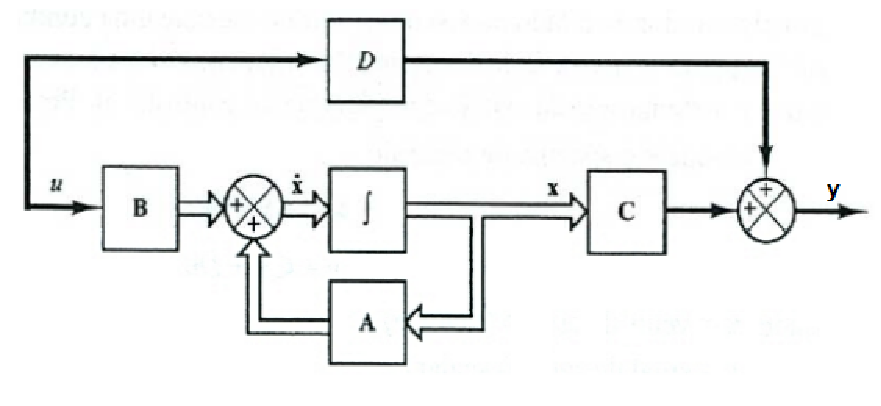
\includegraphics[width=\columnwidth]{./imagens/diagrama1.pdf}
	\renewcommand{\figurename}{Fig.}
    \caption{Sistema de controle no espaço de estados \cite{ogata}.}
	\label{diagrama1}
\end{figure}

\subsubsection{Controlabilidade e Observabilidade}\label{ceo}
Os conceitos de controlabilidade e observabilidade, que possuem importância fundamental no projeto de sistemas de controle por variáveis de estado, foram introduzidos por Kalman \cite{ogata}. Por meio desses conceitos é verificado se existe ou não uma solução completa para certo problema de controle.

Se o sistema for totalmente controlável, significa que a partir de qualquer estado inicial $x(t_0)$ é possível chegar em qualquer estado $x(t)$ esperado, em um tempo finito, por meio de um sinal de controle $u(t)$ \cite{dorf}.

Um sistema é totalmente controlável quando sua matriz de controlabilidade,

\begin{equation}
Cnt=\left[B~|~AB~|~\ldots~|~A^{n-1}B\right]
\end{equation}
é uma matriz quadrada $n\times n$ de determinante $>0$.

O sistema é considerado completamente observável, toda vez que o estado $x(t_0)$ pode ser determinado através da observação de $y(t)$ ao longo de um intervalo de tempo finito. Quando isso acontece, variáveis que não são acessíveis por medição direta podem ser estimadas, e então há a construção dos sinais de controle \cite{ogata}.

Um sistema é totalmente observável quando sua matriz de observabilidade,

\begin{equation}
Obs=\left[C~|~CA~|~\ldots~|~CA^{n-1}\right]^T
\end{equation}
é uma matriz quadrada $n\times n$ de determinante $>0$.

Quando há um sistema totalmente controlável e observável, todos os seus polos em malha fechada podem ser alocados em qualquer região do plano complexo. Desse modo, se torna possível alcançar, no projeto de controladores no espaço de estados, os critérios de desempenho esperados \cite{dorf}.

\subsection{Alocação de Polos em Espaço de Estados}\label{alocacaoEE}
Na realimentação de estados, a fim de gerar um sinal de entrada $u(t)$ para a produção de um sinal de saída $y(t)$ desejado, efetua-se a realimentação de todos os estados $x(t)$. Para que possa ser utilizada essa abordagem, é preciso medir todas as variáveis de estado. Caso isso não seja possível de forma direta, a inclusão de um observador de estados no sistema é necessária \cite{ogata}.

Para o projeto de um controlador por Alocação de Polos em Espaço de Estados, é desejável que o sistema seja totalmente controlável. Nesse caso, os polos de malha fechada do sistema poderão ser alocados em qualquer localização desejada, através da realimentação de estados e da utilização de uma matriz de ganho $K$ correspondente \cite{ogata}.

A aplicação da técnica de projeto por Alocação de Polos começa com a escolha dos polos desejados, baseados em determinadas especificações da reposta natural e/ou da resposta em frequência. Tais especificações podem ser a velocidade, o coeficiente de amortecimento ($\xi$), além da sobrelevação ($M_p$) máxima  e do tempo de estabelecimento ($t_s$) \cite{ogata}.

Supondo que os polos desejados em malha fechada sejam $s=\mu _1$, $s=\mu _2$, $s=\mu _3$, $\ldots$, $s=\mu _n$. Existe uma matriz de ganho $K$ adequada, que é capaz, através da realimentação de estados, de forçar que os polos de malha fechada do sistema se localizem nas posições pretendidas, desde que o sistema seja totalmente controlável \cite{ogata}.

No projeto habitual para sistemas com uma entrada e uma saída (SISO), se projeta um controlador para atender especificações de sobrelevação, $M_p$, e tempo de estabelecimento, $t_s$, e consequentemente de $\xi$ e $\omega _n$, coeficiente de amortecimento e frequência natural de um par de polos complexos.

\begin{equation}\label{mp}
M_p = \exp ^{-\pi\frac{\xi}{\sqrt[]{1-\xi ^2}}}
\end{equation}

\begin{equation}\label{ts3}
t_s = \frac{3}{\xi \omega _n}
\end{equation}
baseado no critério de 3\%, e

\begin{equation}\label{ts5}
t_s = \frac{4}{\xi \omega _n}
\end{equation}
baseado no critério de 5\% \cite{ogata}.

Através das Equações (\ref{mp}), (\ref{ts3}), e (\ref{ts5}) encontram-se as Equações para $\xi$ e $\omega _n$, (\ref{quisi}), (\ref{omegan3}) e (\ref{omegan5}):

\begin{equation}\label{quisi}
\xi = \sqrt[]{\frac{\ln ^2(M_p)}{\pi ^2 + \ln ^2(M_p)}}
\end{equation}

\begin{equation}\label{omegan3}
\omega _n = \frac{3}{\xi t_s}
\end{equation}
baseado no critério de 3\%, e

\begin{equation}\label{omegan5}
\omega _n = \frac{4}{\xi t_s}
\end{equation}
baseado no critério de 5\% \cite{ogata}.

Os polos dominantes do sistema \cite{ogata} são calculados pela Equação (\ref{dominantes}).

\begin{equation}\label{dominantes}
p_{1,2} = -\xi \omega _n \pm \omega _n \sqrt[]{1-\xi ^2}
\end{equation}

Adotando-se o sinal de controle como:

\begin{equation}\label{uEE}
u(t)=-Kx(t)
\end{equation}

Um diagrama de blocos do sistema é apresentado na Figura \ref{diagrama}.
\begin{figure}[H]
	\centering
	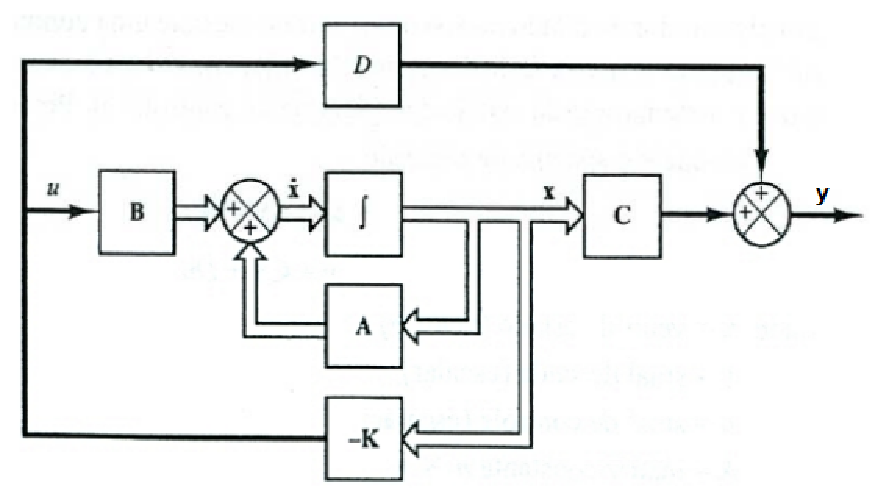
\includegraphics[width=\columnwidth]{./imagens/realimentacaoK.pdf}
	\renewcommand{\figurename}{Fig.}
    \caption{Sistema de controle de malha fechada com $u=-Kx$ \cite{ogata}.}
	\label{diagrama}
\end{figure}

Substituindo o sinal de entrada $u(t)$ nas Equações (\ref{equacaoEstados}) e (\ref{saidaEstados}), podem ser encontradas as equações do sistema em malha fechada. A Equação (\ref{equacaoEstadosMF}) apresenta a equação dos estados, e a Equação (\ref{saidaEstadosMF}) apresenta a equação de saída.

\begin{equation}\label{equacaoEstadosMF}
\dot{x}(t) = (A-BK)x(t)
\end{equation}

\begin{equation}\label{saidaEstadosMF}
y(t)=(C-DK)x(t)
\end{equation}

A solução da equação de estados, Equação (\ref{equacaoEstadosMF}), é dada por:

\begin{equation}\label{solucaoEE}
x(t) = e^{(A-BK)t}x(0)
\end{equation}
com $x(0)$ sendo o estado inicial causado por distúrbios externos. A estabilidade do sistema, bem como a característica da sua resposta no tempo são determinadas pelos autovalores da matriz $A-BK$, que são chamados de polos reguladores. Se eles estiverem posicionados na região do semi-plano esquerdo do plano $s$, a estabilidade do sistema é garantida. Nesse contexto, o problema de alocação de polos consiste em posicionar os polos reguladores do sistema em posições desejadas, através do uso de uma matriz $K$ adequada \cite{ogata}.

\subsubsection{Fórmula de Ackermann para definir a matriz de ganho $K$}
Há uma fórmula conhecida e bastante utilizada para determinar a matriz de ganho $K$, a fórmula de Ackermann \cite{ogata}.

Considere o sistema no espaço de estados
\begin{center}
$\dot{x}=Ax+Bu$,
\end{center}
no qual é feita a utilização de um controle por realimentação de estados, ou seja, a entrada de referência recebe um valor resultante da multiplicação dos estados por ganhos, $u=-Kx$.

Vamos supor que o sistema seja totalmente controlável e que tenha os polos reguladores posicionados em $s=\mu _1$, $s=\mu _2$, $s=\mu _3$, $\ldots$, $s=\mu _n$.

A utilização do controle $u=-Kx$ modifica a equação do sistema, gerando
\begin{center}
$\dot{x}=(A-BK)x$.
\end{center}

Definindo $\tilde{A}=A-BK$, e obtendo a equação característica desejada, onde as raízes são os polos reguladores, temos a Equação (\ref{eqCar}).

\begin{equation}\label{eqCar}
\begin{matrix}
|sI-(A-BK)| = |sI-\tilde{A}| \\= (s-\mu _1)(s-\mu _2)(s-\mu _3)\ldots(s-\mu _n) \\= s^n + \alpha _1 s^{n-1} + \ldots + \alpha _{n-1}s +\alpha _n=0
\end{matrix}
\end{equation}

O Teorema de Cayley Hamilton demonstra que $\tilde{A}$ satisfaz sua própria equação característica \cite{ogata}. Têm-se:

\begin{equation}\label{cayley}
\phi(\tilde{A}) = \tilde{A}^n + \alpha _1 \tilde{A}^{n-1} + \ldots + \alpha _{n-1}\tilde{A} +\alpha _nI=0
\end{equation}

A Equação (\ref{cayley}) será utilizada para a obter a fórmula de Aclermann. Por praticidade de explicação, será considerada a ordem do sistema como $n=3$.

Levando em conta as seguintes identidades:

$I=I$

$\tilde{A} = A-BK$

$\tilde{A}^2 = (A-BK)^2 = A^2-ABK -BK\tilde{A}$

$\tilde{A}^3 = (A-BK)^3 = A^3 - A^2BK -ABK\tilde{A} -BK\tilde{A}^2$

Efetuando a multiplicação das equações anteriores, na mesma ordem, respectivamente por $\alpha _3$, $\alpha _2$, $\alpha _1$ e $\alpha _0$ e somando os resultados, chegamos a:

\begin{equation}\label{multiplicaalfa}
\begin{matrix}
\alpha _3I + \alpha _2 \tilde{A} + \alpha _1 \tilde{A}^2 + \tilde{A}^3\\
= \alpha _3I + \alpha _2 (A-BK) + \alpha _1 (A^2-ABK-BK\tilde{A})\\
+ \tilde{A}^3-A^2BK-ABK\tilde{A}-BK\tilde{A}^2\\
= \alpha _3I + \alpha _2 A + \alpha _1 A^2 + A^3 - \alpha _2BK - \alpha _1ABK \\
- \alpha _1BK\tilde{A} - A^2BK - ABK\tilde{A} - BK\tilde{A}^2\\
\end{matrix}
\end{equation}

Com relação à Equação (\ref{cayley}), têm-se:

\begin{equation}\label{phitildeA}
\tilde{A}^3 + \alpha _1 \tilde{A}^2 + \alpha _2 \tilde{A} +\alpha _3I = \phi(\tilde{A}) = 0
\end{equation}

E também que:

\begin{equation}\label{phiA}
A^3 + \alpha _1 A^2 + \alpha _2 A +\alpha _3I = \phi(A) \neq 0
\end{equation}

Substituindo as Equações (\ref{phitildeA}) e (\ref{phiA}) na Equação (\ref{multiplicaalfa}), chegamos à Equação (\ref{phi}).

\begin{equation}\label{phi}
\begin{matrix}
\phi(\tilde{A})=\phi(A) - \alpha _2BK - \alpha _1ABK \\ - \alpha _1BK\tilde{A} - A^2BK - ABK\tilde{A} - BK\tilde{A}^2
\end{matrix}
\end{equation}

Como $\phi(\tilde{A})=0$, a Equação (\ref{phi}) pode ser reescrita como a Equação (\ref{phiA2}).

\begin{equation}\label{phiA2}
\begin{matrix}
\phi(A)=B(\alpha _2K + \alpha _1K\tilde{A} + K\tilde{A}^2) \\+ AB(\alpha _1K + K\tilde{A}) + A^2BK
\end{matrix}
\end{equation}

E também na forma matricial, como mostra a Equação (\ref{phiA3}).
\begin{equation}\label{phiA3}
\phi(A) = \left[B~|~AB~|~A^2B\right]
\begin{bmatrix}
 \alpha _2K + \alpha _1K\tilde{A} + K\tilde{A}^2 \\ 
 \alpha _1K + K\tilde{A} \\
 K
\end{bmatrix}
\end{equation}

Já que o sistema é totalmente controlável, a matriz inversa da matriz de controlabilidade $\left[B~|~AB~|~A^2B\right]$ existe. Multiplicando os dois lados da Equação (\ref{phiA3}) pela matriz inversa de $\left[B~|~AB~|~A^2B\right]$, obtêm-se a Equação (\ref{multiInversa}).

\begin{equation}\label{multiInversa}
\begin{matrix}
\left[B~|~AB~|~A^2B\right]^{-1}\phi(A)\\ =
\left[\begin{matrix}
 \alpha _2K + \alpha _1K\tilde{A} + K\tilde{A}^2 \\ 
 \alpha _1K + K\tilde{A} \\
 K
\end{matrix}\right]
\end{matrix}
\end{equation}

Multiplicando por $\left[0~0~1\right]$ os dois lados da Equação (\ref{multiInversa}), chegamos na Equação (\ref{multi001}).
\begin{equation}\label{multi001}
\begin{matrix}
\left[0~0~1\right]\left[B~|~AB~|~A^2B\right]^{-1}\phi(A)\\ =
\left[0~0~1\right]
\left[\begin{matrix}
 \alpha _2K + \alpha _1K\tilde{A} + K\tilde{A}^2 \\ 
 \alpha _1K + K\tilde{A} \\
 K
\end{matrix}\right] = K
\end{matrix}
\end{equation}

Reescrevendo a Equação (\ref{multi001}) obtemos:
\begin{equation}\label{multi001dois}
K= \left[0~0~1\right]\left[B~|~AB~|~A^2B\right]^{-1}\phi(A)
\end{equation}

A Equação (\ref{multi001dois}) apresenta a matriz de ganho $K$ de realimentação de estado para um sistema de 3\textordfeminine~ordem.

Para um sistema de ordem $n$, obtemos:
\begin{equation}\label{ackermann}
K= \left[0~0~\ldots~0~1\right]\left[B~|~AB~|\ldots|~A^{n-1}B\right]^{-1}\phi(A)
\end{equation}

A Equação (\ref{ackermann}) é conhecida como fórmula de Ackermann para definição da matriz de ganho $K$ de realimentação de estado \cite{ogata}.

\section{Projeto usando Função de Transferência}\label{funcaotransferencia}
Nesta Seção é apresentado o desenvolvimento do controlador para o sistema utilizando a metodologia de projeto por função de transferência. Nela existem duas subseções, uma correspondente à modelagem matemática do sistema em forma de função de transferência, e a outra ao projeto do controlador.

\subsection{Modelagem do Sistema}\label{modelagem}
Para o projeto, foi utilizado o Sistema de Suspensão Ativa da \textit{Quanser} \cite{quanser}. O modelo matemático do sistema, concedido pelo fabricante, se encontra na Figura \ref{suspensao}.

\begin{figure}[H]
	\centering
	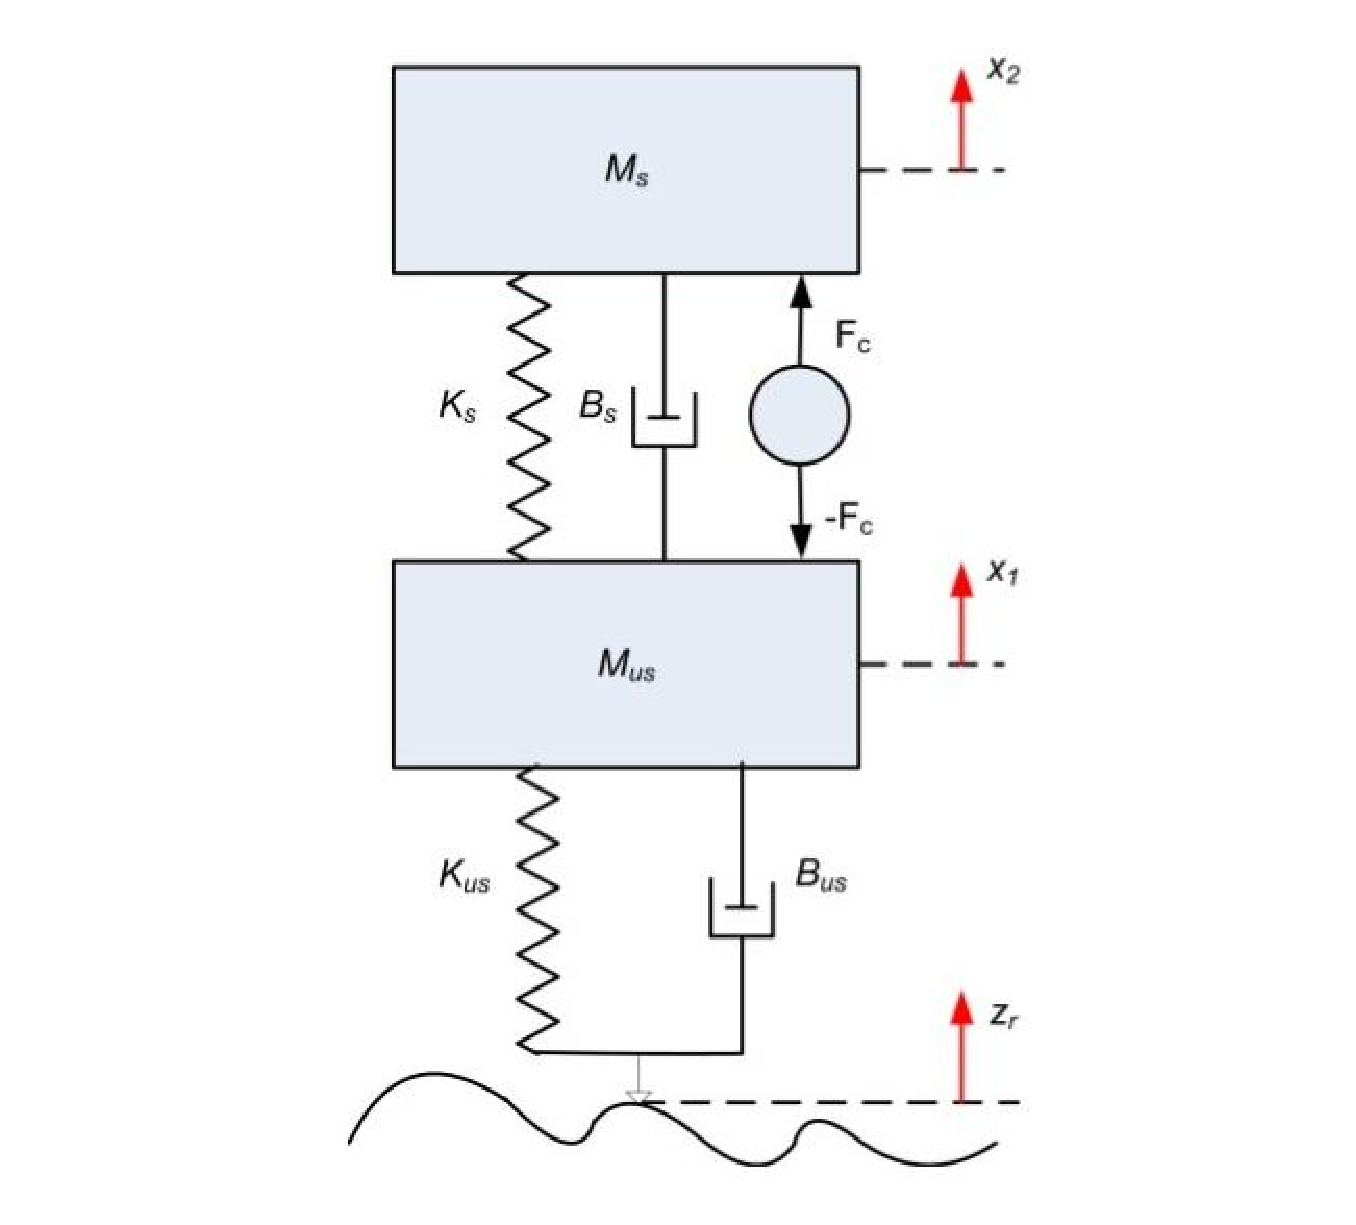
\includegraphics[width=\columnwidth]{./imagens/suspensao.pdf}
    \renewcommand{\figurename}{Fig.}
	\caption{Modelo para o Sistema de Suspensão Ativa da \textit{Quanser} \protect\cite{quanser}.}
	\label{suspensao}
\end{figure}

O Sistema consiste em duas massas móveis suportadas por um par de molas e amortecedores. A massa superior corresponde ao corpo do veículo suportado acima da suspensão, enquanto a massa inferior se refere a uma das rodas do veículo. A ondulação representa a pista.
A modelagem matemática foi possível através da representação do sistema em Equações Diferenciais, as Equações (\ref{x2}) e (\ref{x1}) foram obtidas.

\begin{equation}\label{x2}
\begin{matrix}
\ddot{x_2} = -g + \frac{F_c}{M_s} + \frac{B_s}{M_s}\dot{x_1} - \frac{B_s}{M_s}\dot{x_2} +\\ \frac{K_s}{M_s}x_1 -\frac{K_s}{M_s}x_2
\end{matrix}
\end{equation}

\begin{equation}\label{x1}
\begin{matrix}
\ddot{x_1}= -g - \frac{F_c}{M_{us}} - \frac{B_s+B_us}{M_{us}}\dot{x_1} + \\ \frac{B_{us}}{M_{us}}\dot{x_2} + \frac{B_{us}}{M_{us}}\dot{z_r} - \frac{K_s+K_{us}}{M_{us}}x_1 + \\ \frac{K_s}{M_{us}}x_2 + \frac{K_{us}}{M_{us}}z_r
\end{matrix}
\end{equation}

O sistema é considerado do tipo \textbf{MISO} (Multiple Input, Single Output), possui como entradas a força de controle $F_c$ e a perturbação $z_r$, que representa as ondulações da pista. A força de controle deve ser capaz de minimizar os efeitos causados pela ação da perturbação. A variável a ser controlada é $x_2$, que diz respeito à posição da carroceria do veículo. A variável $x_1$ diz respeito à posição do pneu. A aceleração da gravidade é representada pela constante $g$. Os efeitos da força da gravidade podem ser eliminados, considerando pontos de equilíbrio do sistema. A saída considerada, variável a ser controlada, passa a ser chamada de $z_s$. Os valores numéricos atribuídos a cada parâmetro da Figura \ref{suspensao} são apresentados na Tabela \ref{parametros}.

% \begin{table}[H]{\centering}
% \centering
% 	\caption{Parâmetros do Sistema de Suspensão Ativa}
% 	\begin{tabular}{|c|c|c|} \hline
%    Parâmetro & Valor & Unidade \\ \hline
% 	$M_s$ & 2,45 & kg \\ \hline
%   $M_{us}$ & 1,00 & kg \\ \hline
%   $K_s$ & 900,00 & N/m \\ \hline
%   $K_{us}$ & 1250,00 & N/m \\ \hline
%   $B_s$ & 7,50 & N.s/m \\ \hline
%   $B_{us}$ & 5,00 & N.s/m \\ \hline
%    \end{tabular}
% 	\label{parametros}
% \end{table}
\begin{table}[H]{\centering}
\centering
	\caption{Parâmetros do Sistema de Suspensão Ativa}
	\begin{tabular}{|c|c|c|c|} \hline
   Parâmetro & Identificação & Valor & Unidade \\ \hline
	$M_s$ & Massa do carro & 2,45 & kg \\ \hline
  $M_{us}$ & Massa do pneu & 1,00 & kg \\ \hline
  $K_s$ & Const. de rigidez da suspensão & 900,00 & N/m \\ \hline
  $K_{us}$ & Const. de rigidez do pneu & 1250,00 & N/m \\ \hline
  $B_s$ & Coef. de atrito viscoso da suspensão & 7,50 & N.s/m \\ \hline
  $B_{us}$ & Coef. de atrito viscoso do pneu & 5,00 & N.s/m \\ \hline
   \end{tabular}
	\label{parametros}
\end{table}

Aplicando a Transformada de Laplace podemos obter a resposta em frequência do sistema, ou seja, a representação do mesmo na forma de Função de Transferência. Foram obtidas duas funções, uma relaciona a saída $z_s$ e a força de controle $F_c$, chamada de $G_1(s)$, Equação (\ref{g1}), e a outra relaciona a saída $z_s$ e a perturbação $z_r$, chamada de $G_2(s)$, Equação (\ref{g2}).

\begin{equation}\label{g1}
G_1(s) = \frac{s^2+7,5s+1250}{dG_1(s)}
\end{equation}

\begin{equation}\label{g2}
G_2(s) = \frac{37,5s^2+13875s+1,125e06}{dG_2(s)} 
\end{equation}
Com $dG_1(s)=dG_2(s)=2,45s^4+38,125s^3+6205s^2+13875s+1,125\times10^6$.

Para entender o comportamento do sistema, foi desenvolvida a simulação no \textit{Simulink}. A Figura \ref{mfechada} nos apresenta a resposta natural do sistema em Malha Fechada. Por indicação do fabricante, a perturbação $z_r$ é representada por uma onda quadrada de amplitude 0,01m e frequência 0,3Hz.

\begin{figure}[H]
	\centering
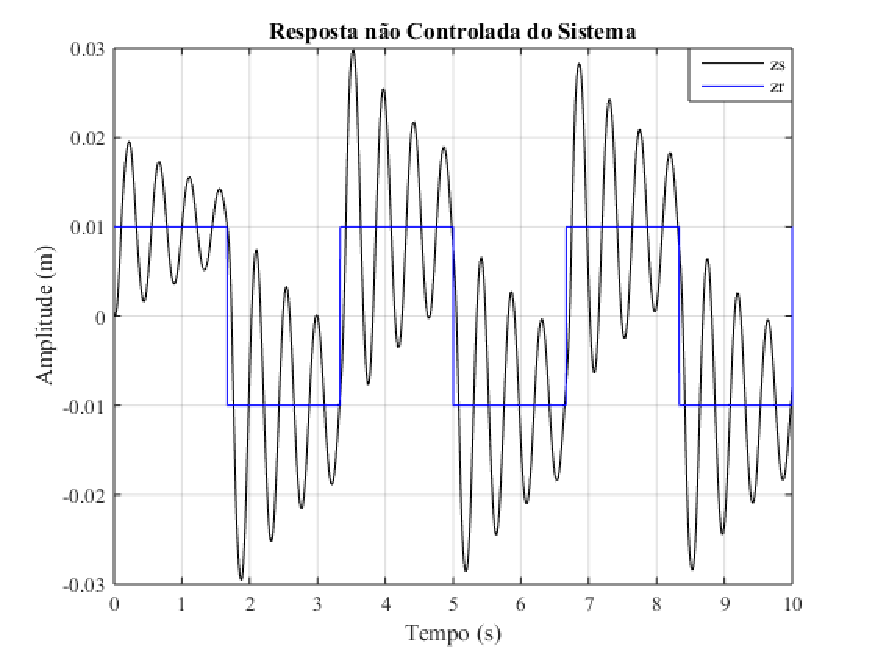
\includegraphics[width=\columnwidth]{./imagens/sistema_malha_fechada.pdf}
	\renewcommand{\figurename}{Fig.}
    \caption{Resposta do Sistema em Malha Fechada.}
	\label{mfechada}
\end{figure}

Através da visualização da Figura \ref{mfechada}, verifica-se que a saída apresenta muita oscilação.

\subsection{Projeto do Controlador}\label{projetoControlador}
A planta possui um atuador responsável por aplicar a força de controle $F_c$, o objetivo é encontrar a equação para o controlador, $G_c(s)$, de modo a minimizar as ondulações geradas pelo efeito da perturbação $z_r$. A Figura \ref{blocos} mostra a disposição dos blocos do sistema controlado.

\begin{figure}[H]
	\centering
	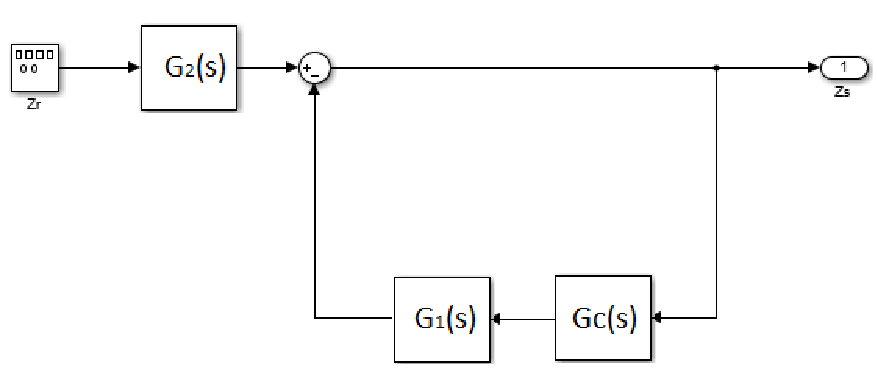
\includegraphics[width=\columnwidth]{./imagens/diagrama_malha_fechada.pdf}
    \renewcommand{\figurename}{Fig.}
    \caption{Diagrama de Blocos do Sistema controlado.}
	\label{blocos}
\end{figure}

Foram feitas diversas tentativas com variados tipos de controladores, podendo ser destacado:

\begin{equation}
G_c(s)=\frac{A_{G_c}s^3+B_{G_c}s^2+C_{G_c}s+D_{G_c}}{E_{G_c}s+F_{G_c}}
\end{equation}

Esse formato de função de transferência para o controlador  proporcionou a mesma quantidade de equações e de coeficientes de $G_c(s)$, condição necessária para que a alocação de polos seja realizada. Foi utilizado controle por Alocação de Polos para encontrar os coeficientes do controlador. O método consiste em escolher o posicionamento dos polos da equação de malha fechada do sistema, e a partir disso, encontrar a equação do denominador de malha fechada, para posteriormente relacioná-la com os coeficientes a serem encontrados para o controlador. A equação de malha fechada é representada pela Equação (\ref{ts}).

%\begin{equation}\label{eqmf}
%T(s) = G_2(s)\frac{1}{1+G_1(s)G_c(s)} 
%\end{equation}
Sendo $G_1(s)=\frac{nG_1(s)}{dG_1(s)}$ e $G_2(s)=\frac{nG_2(s)}{dG_2(s)}$, onde $dG_1(s)=dG_2(s)$ (vide Equações (\ref{g1}) e (\ref{g2})), e $G_c(s)=\frac{nG_c(s)}{dG_c(s)}$. A função $T(s)$ pode ser reescrita como mostra a Equação (\ref{ts1}).

%\begin{equation}\label{seis}
%T(s) = \frac{nG_2(s)}{dG_2 (s)}\frac{1}{\frac{dG_1(s)dG_c(s)+nG_1(s)nG_c(s)}{dG_1(s)dG_c(s)}}
%\end{equation}

Como $dG_1(s)$ e $dG_2(s)$ são iguais, pode-se chamar ambos de $dG(s)$, e $T(s$ passa a ser representada pela Equação (\ref{sete}).

\begin{equation}\label{sete}
T(s) = \frac{nG_2(s)dG(s)dG_c(s)}{dT(s)}
\end{equation}
com $dT(s)=dG(s)dG(s)dG_c(s)+dG(s)nG_1(s)nG_c(s)$.

Depois de efetuar uma simplicação, foi encontrada a Equação (\ref{oito}), que apresenta a função de transferência de malha fechada, $T(s)$.

\begin{equation}\label{oito}
T(s)=\frac{nG_2(s)dG_c(s)}{dG(s)dG_c(s)+nG_1(s)nG_c(s)}
\end{equation}

Para o projeto utilizando como controlador $G_c(s)$, os polos foram alocados com o intuito de eliminar o efeito dos zeros. Foram alocados polos em $s = -250$ e $s = -120$, correspondentes às raízes de $nG_2(s)$ (zeros de $T(s)$ sem o controlador), um par de polos complexos em $s -7,1720+j28,6880$ e $s = -7,1720-j28,6880$, mantendo a parte real do par complexo existente em $dG(s)nG_1(s)$ ($dT(s)$ no sistema sem controlador) e diminuindo sua parte imaginária, ou seja, sua frequência, e alocado também um polo real em $s = -5$, com o intuito de não haver sobrelevação. Com isso o denominador da função de transferência de malha fechada, $dT(s) = (s^2+2\xi \omega_n s+ \omega_n^2)(s+p_1)(s+p_2)(s+p_3)$, pode ser encontrado. A Equação (\ref{dTs}) se refere a $dT(s)$.

\begin{equation}\label{dTs}
\begin{matrix}
dT(s)=s^5+389,344s^4\\+3,8103\times10^4s^3+9,3477\times10^5s^2\\+3,0002\times10^7s+1,3117\times10^8
\end{matrix}
\end{equation}

Conhecendo o denominador de malha fechada, foi possível encontrar os coeficientes do controlador, através da resolução de um sistema de equações lineares, no formato $Aw=b$ (vide Seção \ref{alocacaoFT}). Foram obtidos os seguintes coeficientes para o controlador: $A_{G_c} = -9,531$, $B_{G_c} = 15,42$, $C_{G_c} = 1,885\times10^4$, $D_{G_c} = 1520$, $E_{G_c} = 4,298$, e $F_{G_c} = 114.9$. A matriz $A$ e o vetor $b$ são apresentados nas Equações (\ref{matrizA}) e (\ref{vetorb}). A Equação (\ref{gcs}) se refere a $G_c(s)$.

\begin{equation}\label{matrizA}
A = \begin{bmatrix}
 N_1 & 0 & 0 & 0 & D_1 & 0 \\ 
 N_2 & N_1 & 0 & 0 & D_2 & D_1 \\ 
 N_3 & N_2 & N_1 & 0 & D_3 & D_2 \\ 
 0 & N_3 & N_2 & N_1 & D_4 & D_3 \\
 0 & 0 & N_3 & N_2 & D_5 & D_4 \\
 0 & 0 & 0 & N_3 & 0 & D_5
\end{bmatrix}
\end{equation}
com $N_1=1$, $N_2=7,5$, $N_3=1250$, $D_1=2,45$, $D_2=38,13$, $D_3=6205$, $D_4=13875$, e $D_5=1,125\times10^6$.

O vetor $b$ e o controlador $G_c(s)$ tornam-se:

\begin{equation}\label{vetorb}
b = \begin{bmatrix}
 1 \\ 
 389,344 \\ 
 3,8103\times10^4 \\ 
 9,3477\times10^5 \\
 3,0002\times10^7 \\
 1,3117\times10^8
\end{bmatrix}
\end{equation}

% \begin{equation}\label{gcs}
% G_c(s) = \begin{matrix}
% \frac{-9,531 s^3 + 15,42 s^2 + 1,885\times10^4 s + 1520}{4,298 s + 114,9}
% \end{matrix}
% \end{equation}

\begin{equation}\label{gcs}
G_c(s) = \frac{nG_c(s)}{4,298 s + 114,9}
\end{equation}
onde $nG_c(s)=-9,531 s^3 + 15,42 s^2 + 1,885\times10^4 s + 1520$.

\section{Projeto Usando Espaço de Estados}\label{projetoespacoestados}
Nesta Seção é apresentado o desenvolvimento do controlador para o sistema utilizando a metodologia de projeto por espaço de estados. Nela existem duas subseções, uma correspondente à modelagem matemática do sistema em forma de espaço de estados, e a outra ao projeto do controlador.

\subsection{Modelagem do Sistema}\label{modelagem1}
Na Subseção \ref{espacoestados}, foi apresentada a representação de sistemas no espaço de estados. Foi visto que em malha aberta, a equação de estados e a equação de saída são representadas pelas Equações (\ref{equacaoEstados}) e (\ref{saidaEstados}), respectivamente.

Para o Sistema de Suspensão Ativa, foram definidos como vetor de estados, $x$, vetor de entrada, $u$, e vetor de saída, $y$, apresentados nas Equações (\ref{vetorx}), (\ref{vetoru}), (\ref{vetory}).

\begin{equation}\label{vetorx}
x=\left[ \begin{matrix}
z_s-z_{us} \\
\dot{z_s} \\
z_{us}-z_r \\
\dot{z_{us}}
\end{matrix} \right]
\end{equation}

O primeiro estado representa a deflexão da suspensão, o segundo estado, a velocidade vertical do corpo do veículo, o terceiro estado, a deflexão do pneu, e o quarto estado, a velocidade vertical do pneu \cite{quanser}.

\begin{equation}\label{vetoru}
u=\left[\begin{matrix}
\dot{z_r} \\
F_c
\end{matrix}\right]
\end{equation}

A primeira entrada para o sistema é a velocidade da superfície da estrada, derivada da perturbação $z_r$, a segunda entrada é a força de controle, inicialmente com valor $0$ \cite{quanser}.

\begin{equation}\label{vetory}
y=\left[\begin{matrix}
z_s-z_{us} \\
\ddot{z_s} \\
\end{matrix}\right]
\end{equation}

A primeira saída do sistema é o curso da suspensão, a segunda saída do sistema é a aceleração do corpo (assumindo que o corpo do veículo é equipado com um acelerômetro) \cite{quanser}.

Através das equações diferenciais que representam o sistema, foi possível calcular as matrizes $A$, $B$, $C$ e $D$, dadas pelas Equações (\ref{matriza}), (\ref{matrizb}), (\ref{matrizc}), e (\ref{matrizd}).

\begin{equation}\label{matriza}
A=\left[\begin{matrix}
0 & 1 & 0 & -1 \\
-\frac{K_s}{M_s} & -\frac{B_s}{M_s} & 0 & \frac{B_s}{M_s} \\
0 & 0 & 0 & 1 \\
\frac{K_s}{M_{us}} & \frac{B_s}{M_{us}} & -\frac{K_{us}}{M_{us}} & -\frac{B_s+B_{us}}{M_{us}}
\end{matrix} \right]
\end{equation}

\begin{equation}\label{matrizb}
B=\left[\begin{matrix}
0 & 0 \\
0 & \frac{1}{M_s} \\
-1 & 0 \\
\frac{B_{us}}{M_{us}} & -\frac{1}{M_{us}}
\end{matrix}\right]
\end{equation}

\begin{equation}\label{matrizc}
C=\left[\begin{matrix}
1 & 0 & 0 & 0 \\
-\frac{K_s}{M_s} & -\frac{B_s}{M_s} & 0 & \frac{B_s}{M_s}
\end{matrix}\right]
\end{equation}

\begin{equation}\label{matrizd}
D=\left[ \begin{matrix}
0 & 0 \\
0 & \frac{1}{M_s}
\end{matrix} \right]
\end{equation}

Tendo conhecimento das equações de estado e de saída que representam o sistema, além das matrizes $A$, $B$, $C$ e $D$, foi possível realizar a construção do diagrama de blocos para efetuar a simulação do sistema no \textit{Simulink}. No Apêndice é apresentado o diagrama de blocos do sistema. Com o intuito do projeto em controlar a posição da $z_s$ da suspensão, o uso de dois integradores na segunda saída foi necessário para a visualização dessa variável.

Depois de  efetuada a modelagem, obtendo as equações de estado e de saída, foi possível simular o comportamento do sistema em malha aberta. A Figura \ref{malhaabertaEE} apresenta a resposta natural do sistema, considerando $z_r$ variando de $-0,01$ à $0,01$m, já a Figura \ref{malhaabertaEE2} apresenta a resposta natural do sistema, considerando $z_r$ variando de $0$ à $0,02$m.

\begin{figure}[H]
	\centering
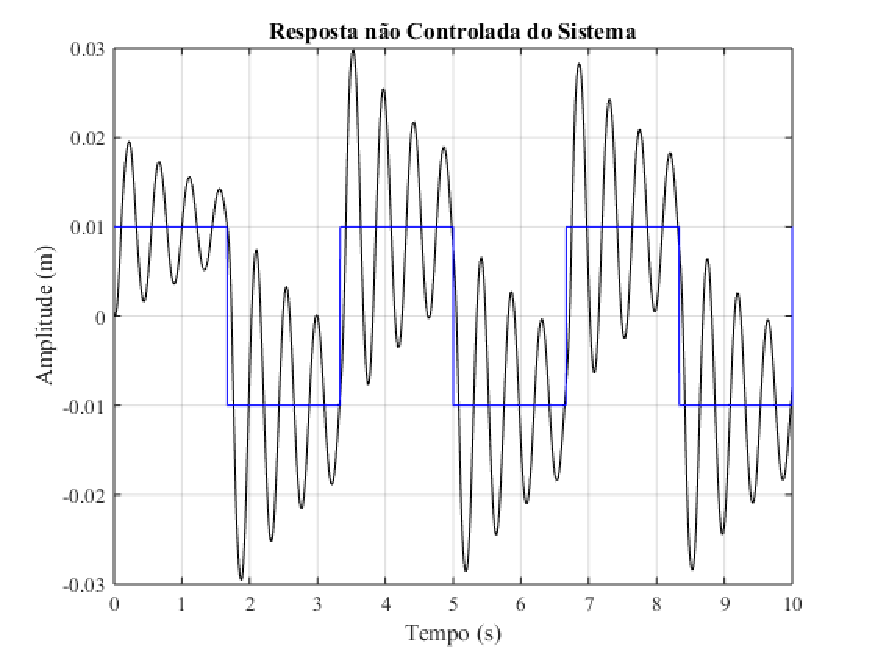
\includegraphics[width=\columnwidth]{./imagens/resposta_natural_sistema.pdf}
	\renewcommand{\figurename}{Fig.}
    \caption{Resposta Natural do Sistema, $z_r$ de $-0,01$ à $0,01$m.}
	\label{malhaabertaEE}
\end{figure}

\begin{figure}[H]
	\centering
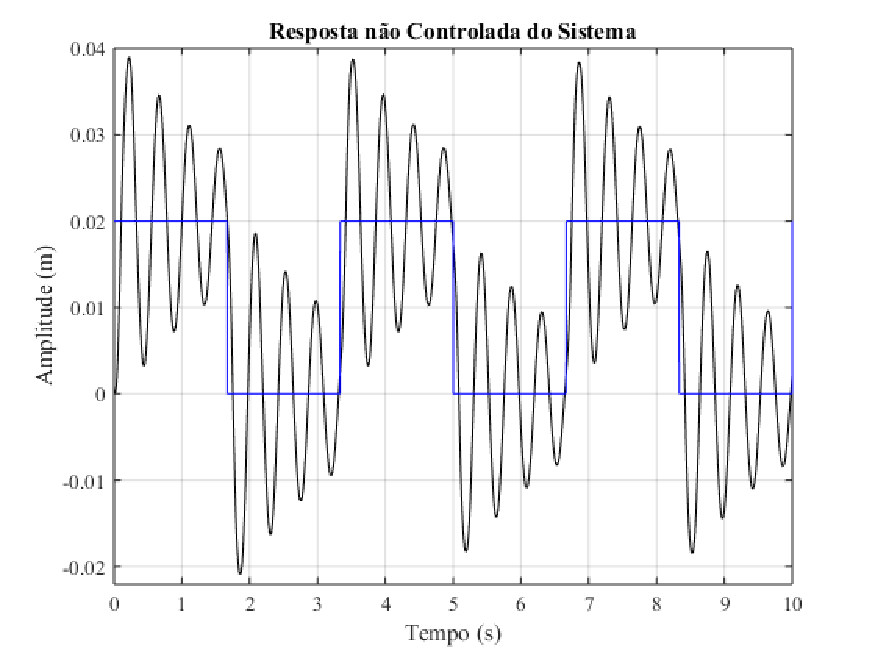
\includegraphics[width=\columnwidth]{./imagens/resposta_natural_sistema2.pdf}
    \renewcommand{\figurename}{Fig.}
    \caption{Resposta Natural do Sistema, $z_r$ de $0$ à $0,02$m.}
	\label{malhaabertaEE2}
\end{figure}

Através da visualização das Figuras \ref{malhaabertaEE} e \ref{malhaabertaEE2}, pode ser verificada a necessidade de uma ação de controle que minimize as oscilações presentes na suspensão, a fim de promover conforto aos passageiros.

\subsection{Projeto do Controlador}\label{projetoControlador1}
O projeto do controlador foi feito baseado na entrada da ação de controle, $F_c$, já que o sistema se apresenta como um regulador, mantêm seu estado atual e, ao sofrer efeito de perturbações, efetua uma ação de controle a fim de retornar a seu estado anterior \cite{ogata}. Através das funções \textit{ctrb} e \textit{obsv} do \textit{matlab} foram verificadas a controlabilidade e a observabilidade do sistema, respectivamente. O sistema se apresentou totalmente controlável e observável.

Com a utilização da função \textit{eig} do \textit{matlab} foi possível conhecer os autovalores da matriz $A$, ou seja, os polos do sistema. Há dois pares de polos complexos, localizados em $p_{1,2}= -0,6087 \pm j14,0644$ e $p_{3,4}=-7,1719 \pm j47,5981$.

Antes de projetar o controlador, foi necessário especificar requisitos de desempenho para o sistema. Foi adotado que a sobrelevação máxima, $M_p$, seria de $5\%$, e o tempo de estabelecimento, $t_s$, seria de $0,5$ segundos.

Baseado na especificação do projeto, foram calculados os valores de $\xi$ e $\omega _n$, através das Equações (\ref{quisi}) e (\ref{omegan5}), e por consequência foram encontrados os polos reguladores do sistema. Os polos dominantes, polos mais próximos do semiplano direito do plano $s$ e que ditam o comportamento do sistema em si (por terem a resposta mais lenta), tem localização em $p_{1,2} = -8 \pm j8,3895$, o outro par de polos foi escolhido em $p_{3,4} = -9,9596 \pm j35,2870$, com intuito de localizá-lo um pouco distante do par de polos dominantes.

Para encontrar a matriz de ganho $K$ através da fórmula de Ackermann, foi utilizada a função \textit{acker} do \textit{matlab}. Ela recebe como parâmetros as matrizes $A$ e $B$ do sistema, além do vetor contendo os polos desejados para o sistema em malha fechada. E como saída nos traz a matriz de ganho $K$. A Equação (\ref{matrizk}) apresenta a matriz $K$ encontrada no projeto.

\begin{equation}\label{matrizk}
K = \left[ \begin{matrix}
-545,9043 & 38,4895 & 45,0246 & -4,6480
\end{matrix} \right]
\end{equation}

\section{Resultados}\label{resultados}
Nesta Seção são apresentados os resultados obtidos por simulações, já que no laboratório ainda não há a planta do sistema em estudo.

\subsection{Projeto usando Função de Transferência}
Conhecendo o controlador e a disposição dos blocos em Malha Fechada, a resposta do sistema controlado pode ser obtida no \textit{matlab}. A Figura \ref{mfechadacontrolada} mostra o resultado dessa simulação. A Figura \ref{sinalcontrole} apresenta o Sinal de Controle resultante da ação de $G_c(s)$.

\begin{figure}[H]
	\centering
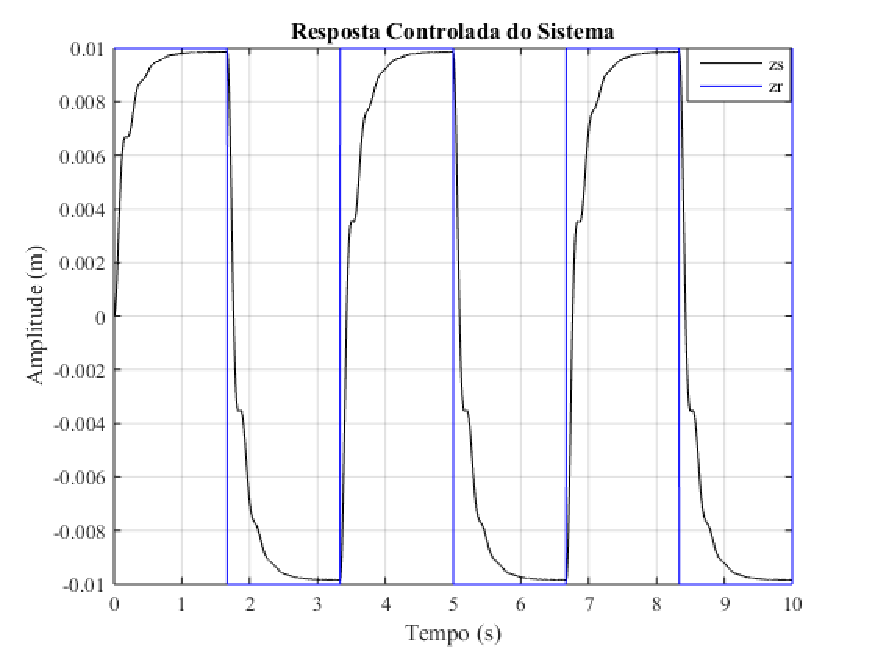
\includegraphics[width=\columnwidth]{./imagens/resposta_controlada.pdf}
    \renewcommand{\figurename}{Fig.}
    \caption{Resposta do Sistema com Controlador.}
	\label{mfechadacontrolada}
\end{figure}

Pode ser verificado que, além de reduzir de forma considerável as oscilações apresentadas pelo sistema, a ação do controlador proporcionou a diminuição do erro de regime, tornando-o quase nulo.

\begin{figure}[H]
	\centering
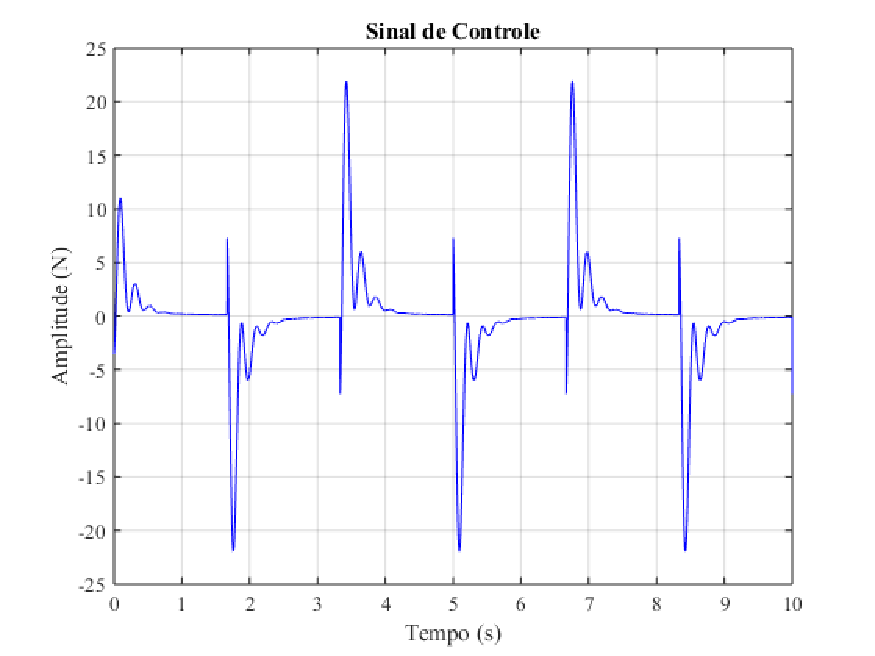
\includegraphics[width=\columnwidth]{./imagens/sinal_de_controle.pdf}
    \renewcommand{\figurename}{Fig.}
    \caption{Sinal de Controle do Sistema.}
	\label{sinalcontrole}
\end{figure}

No que se refere ao Sinal de Controle, foi encontrado um sinal (em módulo) menor que $25$N, e verificando a especificação, vemos que ele está na faixa aceitável, onde ${F_{c}}_{max} = 30$N.

\subsubsection{Teste de Robustez do Controlador $G_c(s)$}
Com o passar do tempo os parâmetros dos sistemas sofrem variações devido ao desgaste dos componentes do sistema. Tais componentes passam a apresentar valores diferentes dos identificados inicialmente. Por esse motivo, se torna importante avaliar o comportamento de um controlador em casos de variação de parâmetros.

Para testar a robustez do controlador $G_c(s)$, Equação (\ref{gcs}), obtido na Seção \ref{projetoControlador} foram aplicadas variações nos parâmetros da planta e efetuadas as simulações para obtenção e análise das respostas encontradas.

Após a variação, os parâmetros passam a representar intervalos, e não um valor escalar. Será avaliado o comportamento do sistema em malha fechada e do controlador, levando em consideração os diversos valores apresentados pelos parâmetros da planta.

No primeiro caso foram levadas em consideração as variações de $K_s$ e $K_{us}$ em 3\%, e de $B_s$ e $B_{us}$ em 10\%.

%Com isso os novos valores desses parâmetros são: $K_s$ = [873,~927] N/m, $K_{us}$ = [1212,5,~1287,5] N/m, $B_s$ = [6,75,~8,25] N.s/m e $B_{us}$ = [4,5,~5,5] N.s/m. Os outros parâmetros apresentam os valores referentes aos da Tabela \ref{parametros}.

Os valores numéricos atualizados atribuídos a cada parâmetro são apresentados na Tabela \ref{parametros1}.

\begin{table}[H]{\centering}
\centering
	\caption{Parâmetros do Sistema de Suspensão Ativa}
	\begin{tabular}{|c|c|c|} \hline
    Parâmetro & Valor & Unidade \\ \hline
    $M_s$ & 2,45 & kg \\ \hline
    $M_{us}$ & 1,00 & kg \\ \hline
    $K_s$ & [873,00,~927,00] & N/m \\ \hline
    $K_{us}$ & [1212,50,~1287,50] & N/m \\ \hline
    $B_s$ & [6,75,~8,25] & N.s/m \\ \hline
    $B_{us}$ & [4,50,~5,50] & N.s/m \\ \hline
   \end{tabular}
	\label{parametros1}
\end{table}

Para a simulação, foram utilizados 7 valores do intervalo de cada parâmetro que sofreu variação, totalizando 2401 iterações. A Tabela \ref{caso1} apresenta os 7 valores considerados para $K_s$, $K_{us}$, $B_s$ e $B_{us}$.

\begin{table}[H]{\centering}
\centering
    \caption{Valores Utilizados para os Parâmetros dentro do Intervalo}
    \begin{tabular}{|c|c|c|c|c|} \hline
        Valor & $K_s$ & $K_{us}$ & $B_s$ & $B_{us}$ \\ \hline
        1 & 873,00 & 1212,50 & 6,75 & 4,50 \\ \hline
        2 & 882,00 & 1225,00 & 7,00 & 4,67 \\ \hline
        3 & 891,00 & 1237,50 & 7,25 & 4,83 \\ \hline
        4 & 900,00 & 1250,00 & 7,50 & 5,00 \\ \hline
        5 & 909,00 & 1262,50 & 7,75 & 5,17 \\ \hline
        6 & 918,00 & 1275,00 & 8,00 & 5,33 \\ \hline
        7 & 927,00 & 1287,50 & 8,25 & 5,50 \\ \hline
    \end{tabular}
    \label{caso1}
\end{table}

A Figura \ref{sistemaIntervalar} traz as várias respostas do Sistema, sem a presença do controlador, com variação dos parâmetros, em Malha Fechada.
\begin{figure}[H]
	\centering
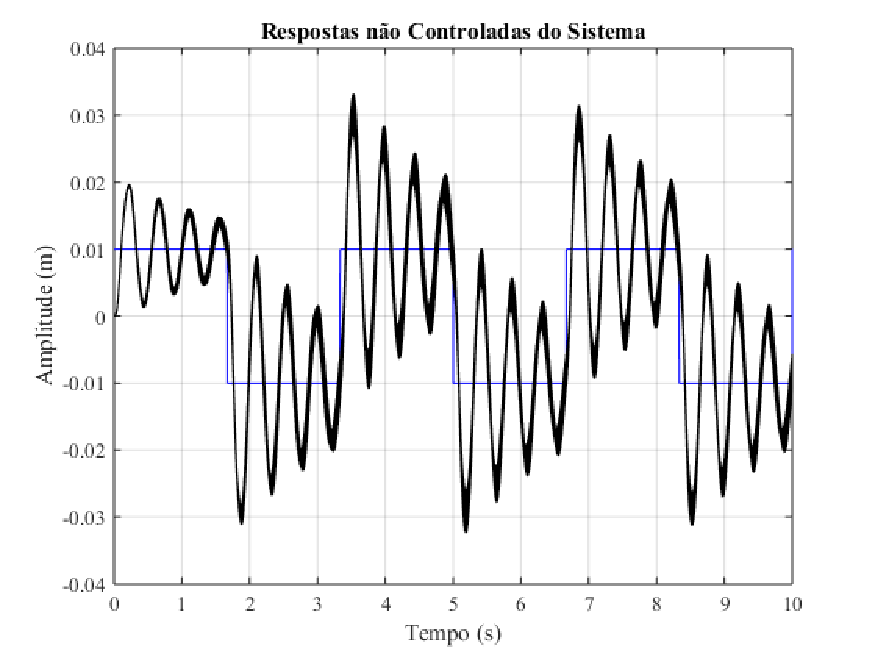
\includegraphics[width=\columnwidth]{./imagens/resposta_sistema_variando_Ks_Kus_Bs_Bus.pdf}
    \renewcommand{\figurename}{Fig.}
    \caption{Respostas não Controladas do Sistema com variação de $K_s$ e $K_{us}$ em 3\%, e $B_s$ e $B_{us}$ em 10\%.}
	\label{sistemaIntervalar}
\end{figure}

A Figura \ref{controladaIntervalar} apresenta as respostas do Sistema, com a ação do controlador $G_c(s)$.
\begin{figure}[H]
	\centering
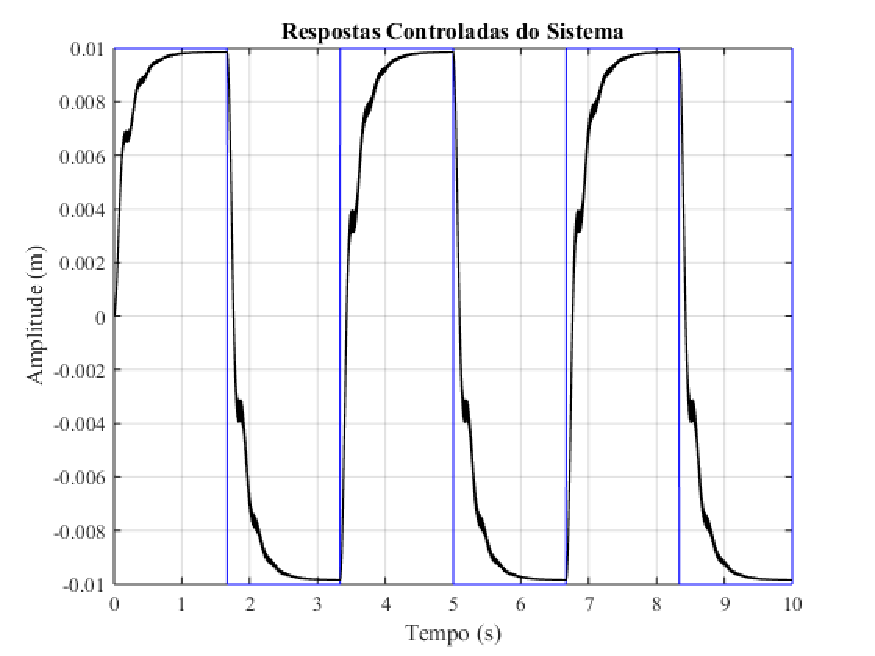
\includegraphics[width=\columnwidth]{./imagens/resposta_controlada_variando_Ks_Kus_Bs_Bus_controlador_sem_robustez.pdf}
    \renewcommand{\figurename}{Fig.}
    \caption{Respostas Controladas do Sistema com variação de $K_s$ e $K_{us}$ em 3\%, e $B_s$ e $B_{us}$ em 10\%.}
	\label{controladaIntervalar}
\end{figure}

A Figura \ref{sinalcontroleIntervalar} mostra os vários Sinais de Controle resultantes da ação de $G_c(s)$ e a variação de parâmetros da planta.
\begin{figure}[H]
	\centering
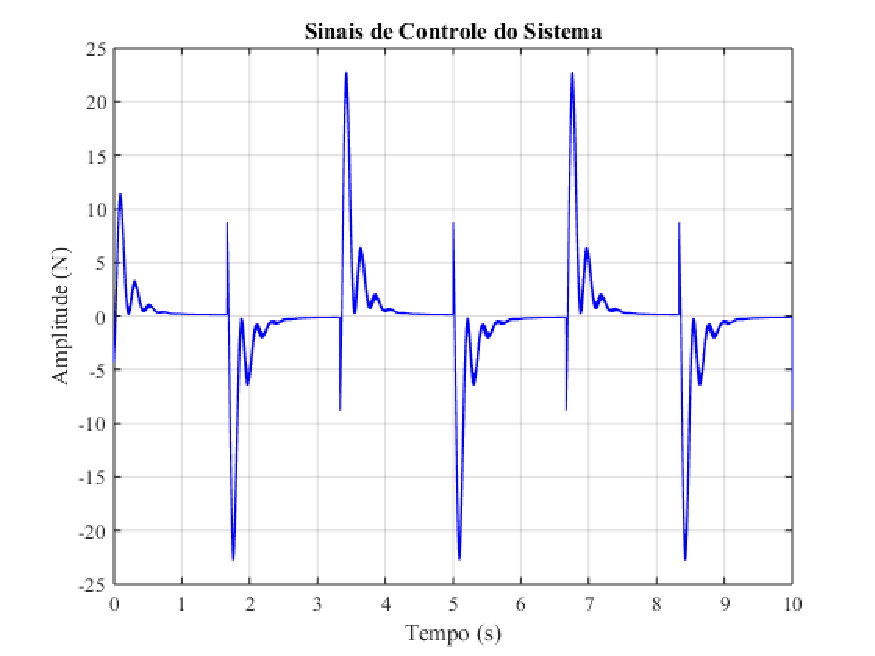
\includegraphics[width=\columnwidth]{./imagens/sinal_de_controle_variando_Ks_Kus_Bs_Bus_controlador_sem_robustez.pdf}
	\renewcommand{\figurename}{Fig.}
    \caption{Sinais de Controle do Sistema com variação de $K_s$ e $K_{us}$ em 3\%, e $B_s$ e $B_{us}$ em 10\%.}
	\label{sinalcontroleIntervalar}
\end{figure}

No segundo caso foram levadas em consideração as variações de $K_s$ e $K_{us}$ em 5\%, e de $B_s$ e $B_{us}$ em 10\%. 

%Com isso os novos valores desses parâmetros são: $K_s$ = [855,~945] N/m, $K_{us}$ = [1187,5,~1312,5] N/m, $B_s$ = [6,75,~8,25] N.s/m e $B_{us}$ = [4,5,~5,5] N.s/m. Os outros parâmetros apresentam os valores referentes aos da Tabela \ref{parametros}.

Os valores numéricos atualizados atribuídos a cada parâmetro são apresentados na Tabela \ref{parametros2}.

\begin{table}[H]{\centering}
\centering
	\caption{Parâmetros do Sistema de Suspensão Ativa}
	\begin{tabular}{|c|c|c|} \hline
   Parâmetro & Valor & Unidade \\ \hline
	$M_s$ & 2,45 & kg \\ \hline
  $M_{us}$ & 1,00 & kg \\ \hline
  $K_s$ & [855,00,~945,00] & N/m \\ \hline
  $K_{us}$ & [1187,50,~1312,50] & N/m \\ \hline
  $B_s$ & [6,75,~8,25] & N.s/m \\ \hline
  $B_{us}$ & [4,50,~5,50] & N.s/m \\ \hline
   \end{tabular}
	\label{parametros2}
\end{table}

Para essa simulação, também foram utilizados 7 valores do intervalo de cada parâmetro que sofreu variação, realizando um total de 2401 iterações. A Tabela \ref{caso2} apresenta os 7 valores considerados para $K_s$, $K_{us}$, $B_s$ e $B_{us}$.

\begin{table}[H]{\centering}
\centering
    \caption{Valores Utilizados para os Parâmetros dentro do Intervalo}
    \begin{tabular}{|c|c|c|c|c|} \hline
        Valor & $K_s$ & $K_{us}$ & $B_s$ & $B_{us}$ \\ \hline
        1 & 855,00 & 1187,50 & 6,75 & 4,50 \\ \hline
        2 & 870,00 & 1208,33 & 7,00 & 4,67 \\ \hline
        3 & 885,00 & 1229,17 & 7,25 & 4,83 \\ \hline
        4 & 900,00 & 1250,00 & 7,50 & 5,00 \\ \hline
        5 & 915,00 & 1270,83 & 7,75 & 5,17 \\ \hline
        6 & 930,00 & 1291,67 & 8,00 & 5,33 \\ \hline
        7 & 945,00 & 1312,50 & 8,25 & 5,50 \\ \hline
    \end{tabular}
    \label{caso2}
\end{table}

A Figura \ref{sistemaIntervalar2} traz as várias respostas do Sistema, sem a presença do controlador, com variação dos parâmetros, em Malha Fechada.
\begin{figure}[H]
	\centering
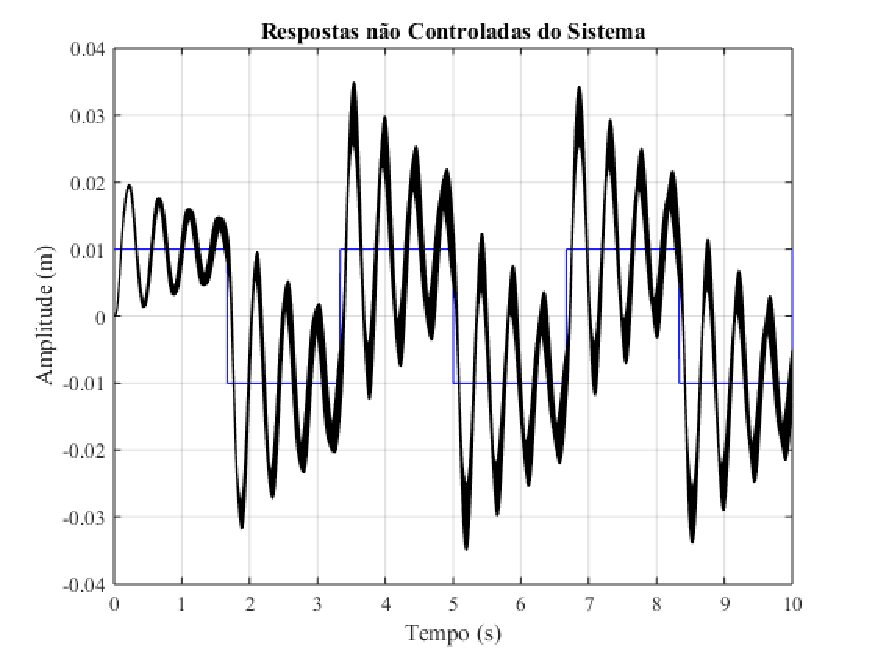
\includegraphics[width=\columnwidth]{./imagens/resposta_sistema_variando_Ks_Kus_5_Bs_Bus_10.pdf}
    \renewcommand{\figurename}{Fig.}
    \caption{Respostas não Controladas do Sistema com variação de $K_s$ e $K_{us}$ em 5\%, e $B_s$ e $B_{us}$ em 10\%.}
	\label{sistemaIntervalar2}
\end{figure}

A Figura \ref{controladaIntervalar2} apresenta as respostas do Sistema, com a ação do controlador $G_c(s)$.
\begin{figure}[H]
	\centering
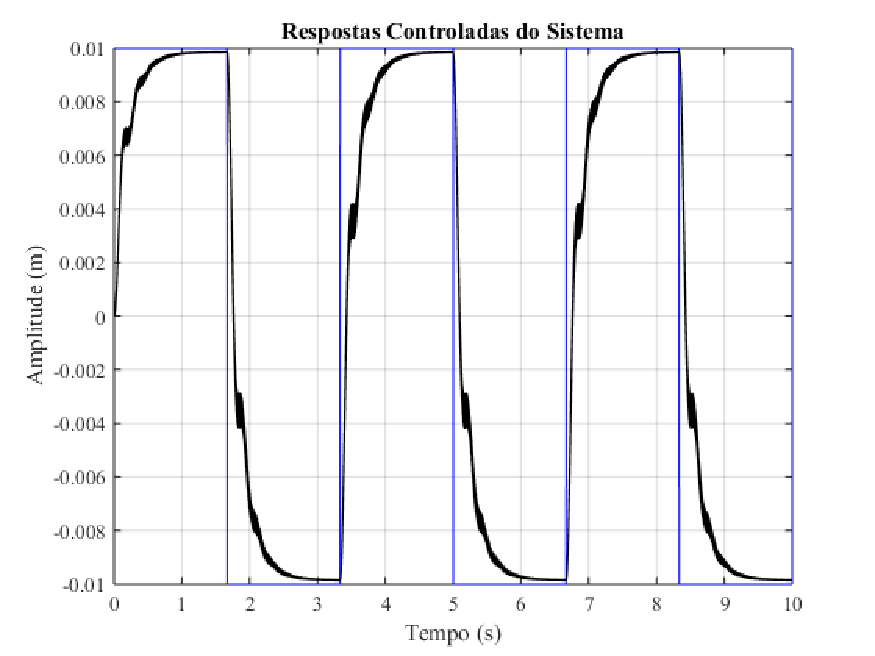
\includegraphics[width=\columnwidth]{./imagens/resposta_controlada_variando_Ks_Kus_5_Bs_Bus_10_controlador_sem_robustez.pdf}
    \renewcommand{\figurename}{Fig.}
    \caption{Respostas Controladas do Sistema com variação de $K_s$ e $K_{us}$ em 5\%, e $B_s$ e $B_{us}$ em 10\%.}
	\label{controladaIntervalar2}
\end{figure}

A Figura \ref{sinalcontroleIntervalar2} mostra os vários Sinais de Controle resultantes da ação de $G_c(s)$ e a variação de parâmetros da planta.
\begin{figure}[H]
	\centering
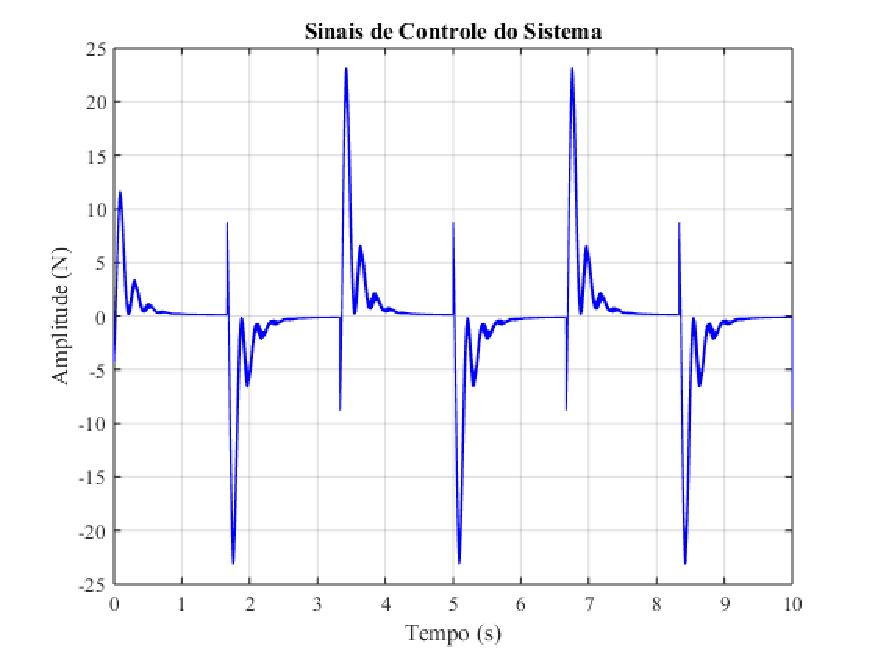
\includegraphics[width=\columnwidth]{./imagens/sinal_de_controle_variando_Ks_Kus_5_Bs_Bus_10_controlador_sem_robustez.pdf}
    \renewcommand{\figurename}{Fig.}
    \caption{Sinais de Controle do Sistema com variação de $K_s$ e $K_{us}$ em 5\%, e $B_s$ e $B_{us}$ em 10\%.}
	\label{sinalcontroleIntervalar2}
\end{figure}

Nos dois casos de variação dos parâmetros, assim como no resultado obtido sem a variação, pode ser verificado que as oscilações apresentadas pelo sistema foram diminuídas de forma considerável, e também que a ação do controlador proporcionou a diminuição do erro de regime.

No que se refere ao Sinal de Controle, o resultado também foi satisfatório, mais uma vez foi encontrado um sinal (em módulo) menor que $25$N, e por consequência $< 30$N.

\subsection{Projeto usando Espaço de Estados}
Conhecendo a matriz de ganho $K$, pode ser feita a realimentação $u=-Kx$, com $u=F_c$. A Figura \ref{malhafechadaEE} apresenta a resposta controlada do sistema, a Figura \ref{sinalcontroleEE} mostra o esforço de controle para alocar os polos nas posições desejadas, considerando $z_r$ de $-0,01$ a $0,01$m.

\begin{figure}[H]
	\centering
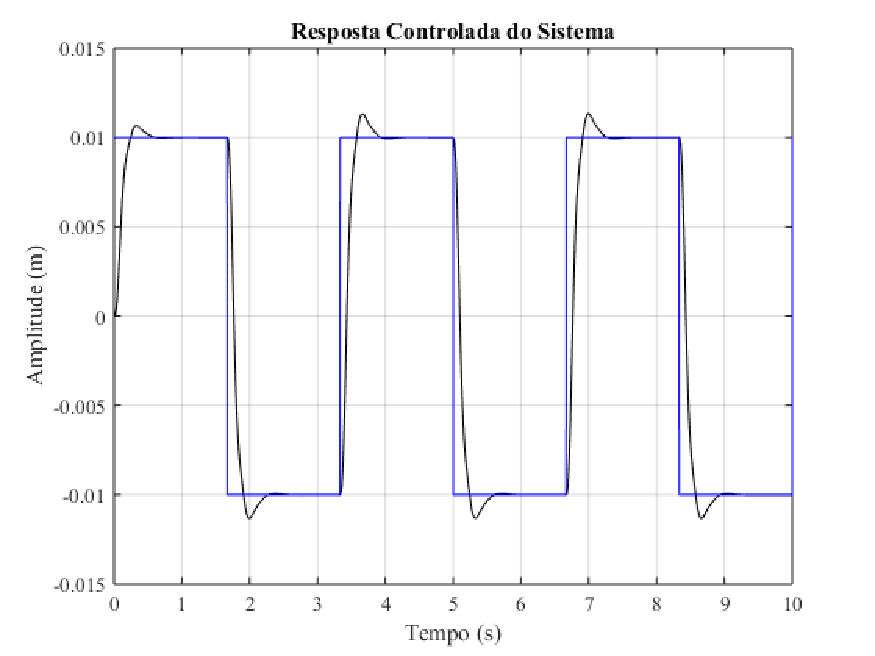
\includegraphics[width=\columnwidth]{./imagens/resposta_controlada_sistema.pdf}
    \renewcommand{\figurename}{Fig.}
    \caption{Resposta Controlada do Sistema, $z_r$ de $-0,01$ à $0,01$m.}
	\label{malhafechadaEE}
\end{figure}
A resposta aponta um $M_p$ de aproximadamente 7,5\% e um $t_s$ de aproximadamente $0,4$ segundos. Acredita-se que a influência do segundo par de polos complexos fez com que as especificações não fossem totalmente atendidas.

\begin{figure}[H]
	\centering
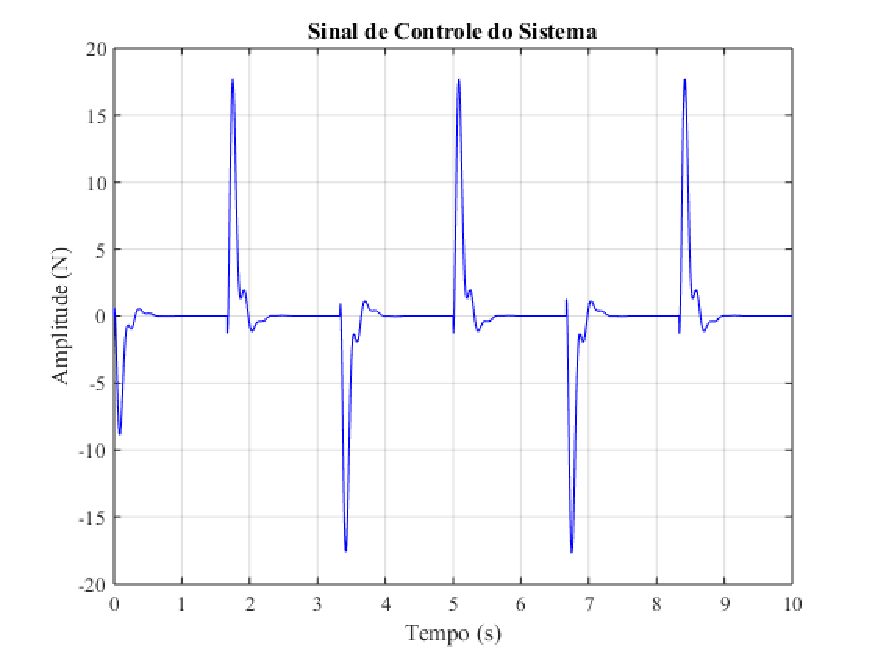
\includegraphics[width=\columnwidth]{./imagens/sinal_controle_sistema.pdf}
    \renewcommand{\figurename}{Fig.}
    \caption{Sinal de Controle do Sistema, $z_r$ de $-0,01$ à $0,01$m.}
	\label{sinalcontroleEE}
\end{figure}
A ação do controlador apresentou um máximo sinal de controle menor que $20$N, valor que pertence à faixa de $\pm 30$N, que é a faixa limite permitida.

A Figura \ref{malhafechadaEE2} apresenta a resposta controlada do sistema, a Figura \ref{sinalcontroleEE2} mostra o esforço de controle para alocar os polos nas posições desejadas, considerando $z_r$ de $0$ a $0,02$m.

\begin{figure}[H]
	\centering
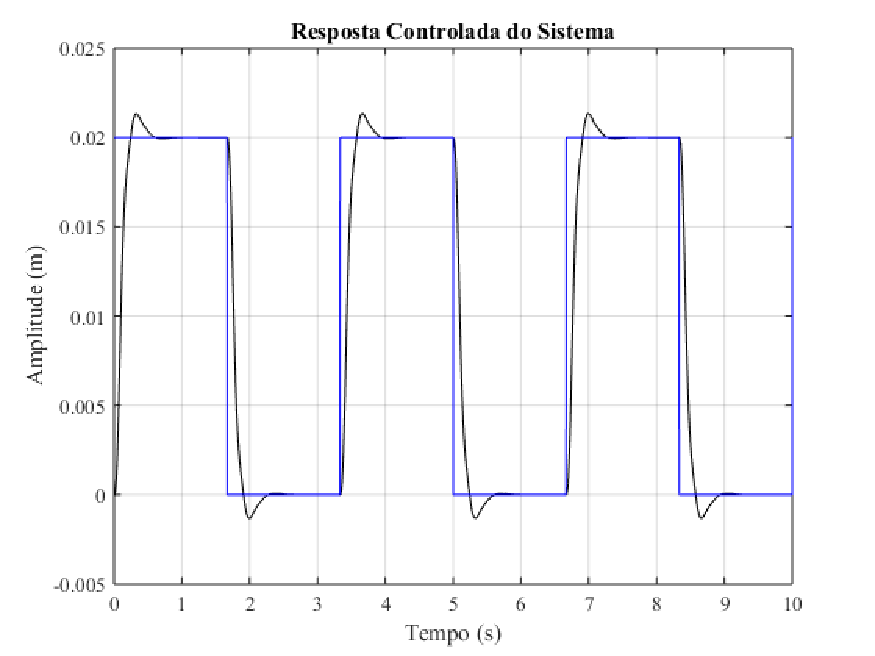
\includegraphics[width=\columnwidth]{./imagens/resposta_controlada_sistema2.pdf}
    \renewcommand{\figurename}{Fig.}
    \caption{Resposta Controlada do Sistema, $z_r$ de $0$ à $0,02$m.}
	\label{malhafechadaEE2}
\end{figure}

Essa resposta também aponta um $M_p$ de aproximadamente 7,5\% e um $t_s$ de aproximadamente $0,4$ segundos. Assim como na simulação anterior, acredita-se que a influência do segundo par de polos complexos fez com que as especificações não fossem totalmente atendidas.

\begin{figure}[H]
	\centering
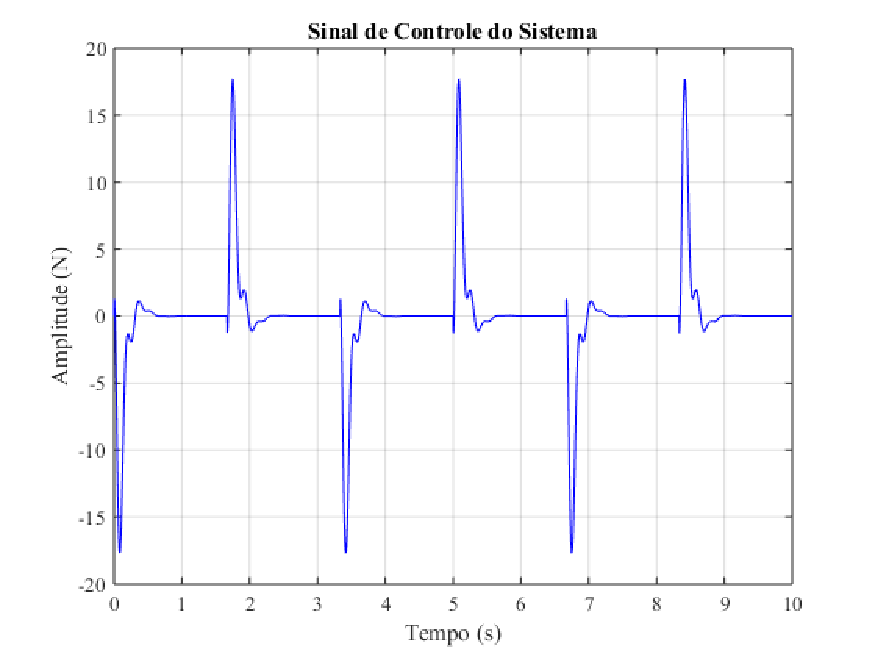
\includegraphics[width=\columnwidth]{./imagens/sinal_controle_sistema2.pdf}
    \renewcommand{\figurename}{Fig.}
    \caption{Sinal de Controle do Sistema, $z_r$ de $0$ à $0,02$m.}
	\label{sinalcontroleEE2}
\end{figure}
A ação do controlador nessa simulação também apresentou um máximo sinal de controle menor que $20$N, valor que pertence à faixa de $\pm 30$N, que é a faixa limite permitida.

Na Guia de Laboratório do Sistema de Suspensão Ativa, fornecido pela \textit{Quanser}, há o projeto de um controlador por realimentação de estados. Nesse projeto é encontrada uma matriz de ganho $K =
\left[\begin{matrix}
24,66 & 48,87 & -0,47 & 3,68
\end{matrix}\right]$ \cite{quanser}.

A Figura \ref{quanserE} apresenta a resposta controlada do sistema, a Figura \ref{quanserE2} mostra o esforço de controle, utilizando essa matriz $K$ para a realimentação, considerando $z_r$ de $-0,01$ à $0,01$m.

\begin{figure}[H]
	\centering
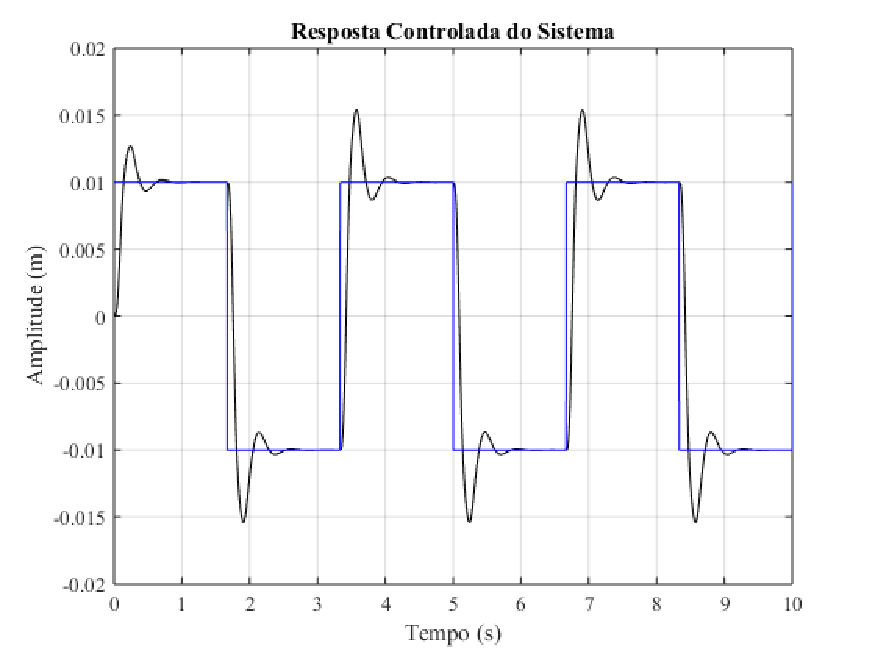
\includegraphics[width=\columnwidth]{./imagens/quanserE.pdf}
    \renewcommand{\figurename}{Fig.}
    \caption{Resposta Controlada do Sistema, $z_r$ de $-0,01$ à $0,01$m.}
	\label{quanserE}
\end{figure}
A resposta aponta um $M_p$ de aproximadamente 25,4\% e um $t_s$ de aproximadamente $0,525$ segundos.

\begin{figure}[H]
	\centering
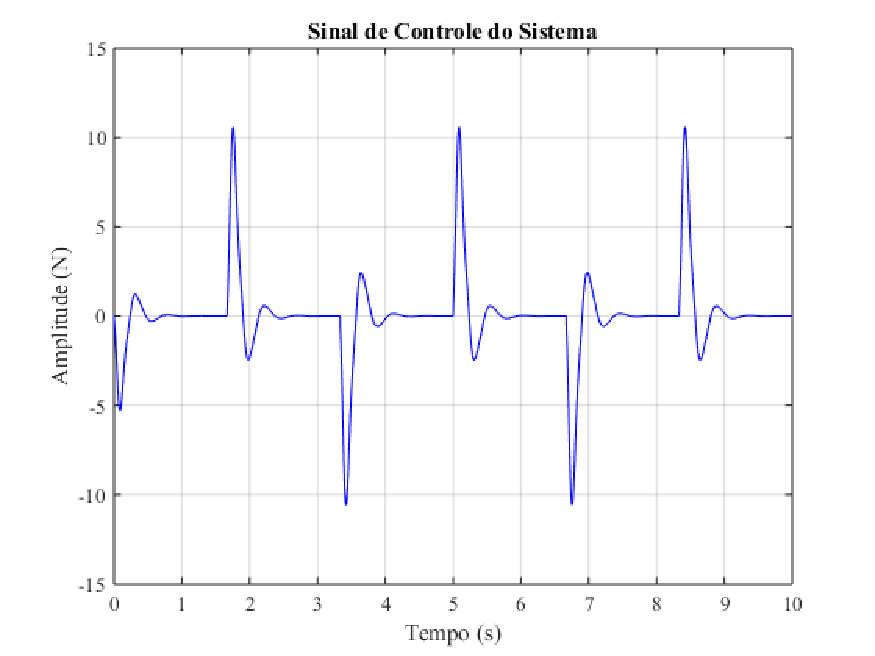
\includegraphics[width=\columnwidth]{./imagens/quanserE2.pdf}
    \renewcommand{\figurename}{Fig.}
    \caption{Sinal de Controle do Sistema, $z_r$ de $-0,01$ à $0,01$m.}
	\label{quanserE2}
\end{figure}
A ação do controlador apresentou um máximo sinal de controle menor que $15$N, valor que pertence à faixa de $\pm 30$N, que é a faixa limite permitida.

A Figura \ref{quanserEE} apresenta a resposta controlada do sistema, a Figura \ref{quanserEE2} mostra o esforço de controle, utilizando essa matriz $K$ para a realimentação, considerando $z_r$ de $0$ à $0,02$m.

\begin{figure}[H]
	\centering
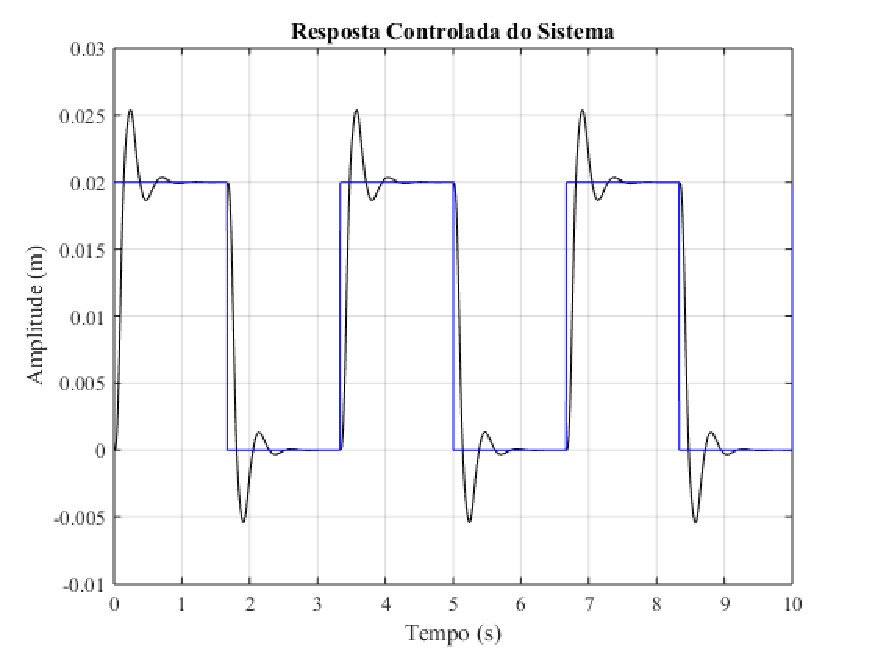
\includegraphics[width=\columnwidth]{./imagens/quanserEE.pdf}
    \renewcommand{\figurename}{Fig.}
    \caption{Resposta Controlada do Sistema, $z_r$ de $0$ à $0,02$m.}
	\label{quanserEE}
\end{figure}
Essa resposta também aponta um $M_p$ de aproximadamente 25,4\% e um $t_s$ de aproximadamente $0,525$ segundos.

\begin{figure}[H]
	\centering
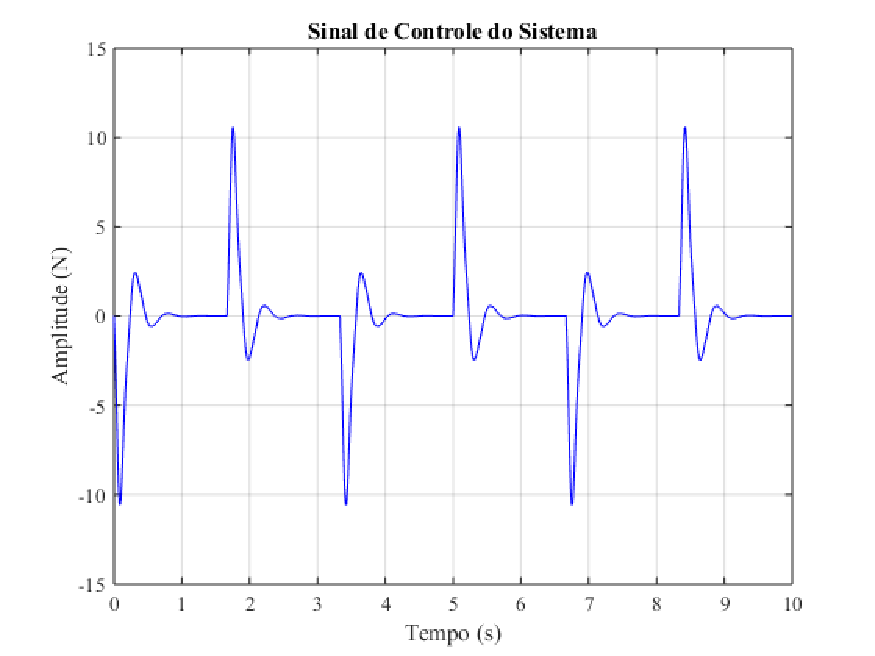
\includegraphics[width=\columnwidth]{./imagens/quanserEE2.pdf}
    \renewcommand{\figurename}{Fig.}
    \caption{Sinal de Controle do Sistema, $z_r$ de $0$ à $0,02$m.}
	\label{quanserEE2}
\end{figure}
A ação do controlador nessa simulação também apresentou um máximo sinal de controle menor que $15$N, valor que pertence à faixa de $\pm 30$N, que é a faixa limite permitida.

\section{Conclusões}\label{conclusao}
Analisando os resultados obtidos com os projetos dos controladores por Alocação de Polos, foi possível perceber que tanto no projeto por função de transferência como no projeto por realimentação de estados, houve o atendimento das especificações do projeto, no que diz respeito à minimização das oscilações do veículo.

O projeto por função de transferência não apresentou sobrelevação, e apresentou um tempo de estabelecimento de $0,75$ segundos. O projeto por realimentação de estados apresentou uma sobrelevação máxima de $7,5$\%, e um tempo de estabelecimento de $0,4$ segundos. Além disso, em ambos os casos, vimos que o sinal de controle apresentou valores dentro do esperado.

O projeto do controlador por Alocação de Polos usando função de transferência se mostrou eficaz, visto que mesmo considerando variações nos parâmetros da planta, a ação do controlador obtido resultou no atendimento das especificações.

No projeto com função de transferência, foram feitas tentativas de aplicar a Análise Intervalar Modal \cite{modal} para efetuar o projeto de controladores robustos \cite{prado2008controle} para o Sistema de Suspensão Ativa, mas não foram obtidos resultados satisfatórios.

Comparando os resultados obtidos no projeto com realimentação de estados com os resultados alcançados no manual da \textit{Quanser}, podem ser constatados menores valores para o $M_p$ e para o $t_s$ no projeto desenvolvido neste trabalho. Em relação ao esforço de controle, o do controlador obtido no manual da \textit{Quanser} apresentou valor menor, e os dois projetos apresentaram valores pertencentes à faixa permitida.

Como  trabalho  futuro pode ser citado o projeto de controladores robustos via programação alvo para o Sistema de Suspensão Ativa, considerando o sistema com Realimentação de Estados, utilizando a metodologia proposta por \cite{lordelo}. Além disso, poderia se fazer a implementação prática do controlador no sistema real caso se conseguisse obter a planta do sistema.

\onecolumn
\appendix[Modelo do Sistema de Suspensão Ativa no \textit{Simulink}]\label{apendice}

\begin{figure}[H]
	\centering
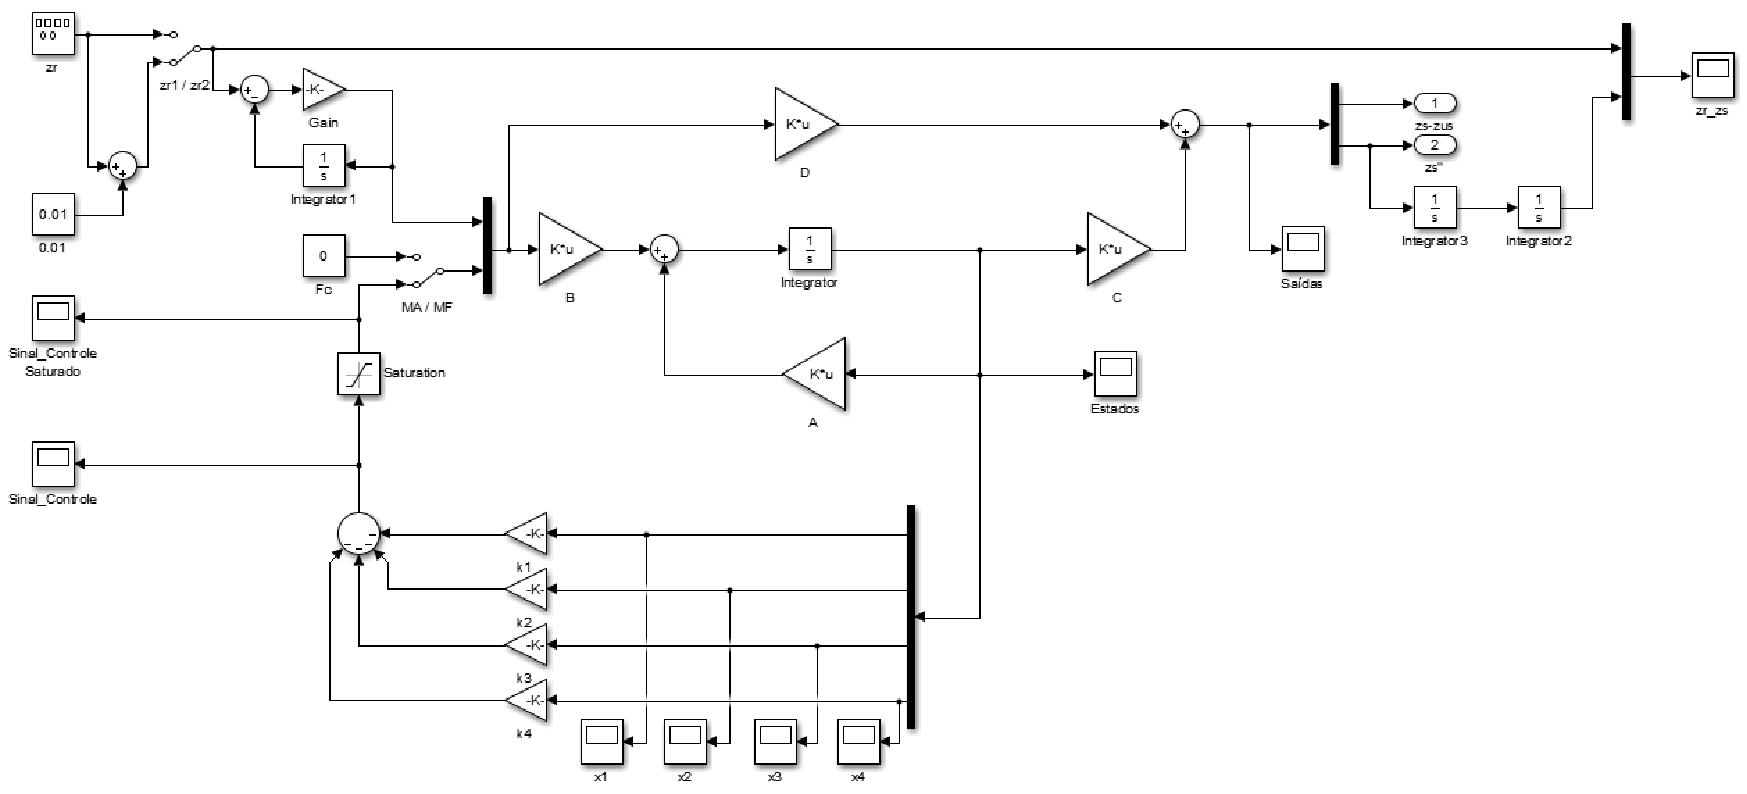
\includegraphics[width=\columnwidth]{./imagens/modeloSimulink_malha_fechada.pdf}
    \renewcommand{\figurename}{Fig.}
    \caption{Diagrama de Blocos do Sistema de Suspensão Ativa.}
	\label{modeloSimulink2}
\end{figure}

\begin{multicols}{2}
\section*{Agradecimentos}
Agradeço Deus pela vida e pela família que me deu. Aos meus pais, Maria Bárbara e João, e à minhas irmãs, por todo incentivo e apoio durante minha trajetória. Agradeço a todos os meus amigos e companheiros de estudo, e aos demais colegas de curso, por todo aprendizado compartilhado e toda ajuda. E também pelos momentos de diversão tidos nesses últimos anos. Agradeço a todos os meus professores, em especial à minha orientadora, Márcia Lissandra Machado Prado, por toda dedicação e esforço no acompanhamento durante os dois anos de desenvolvimento deste trabalho, e por ter me apresentado o mundo dos sistemas de controle.

\bibliographystyle{IEEEtran}
\bibliography{./bibtex/bib/referencia}

\begin{figure}[H]
	\centering
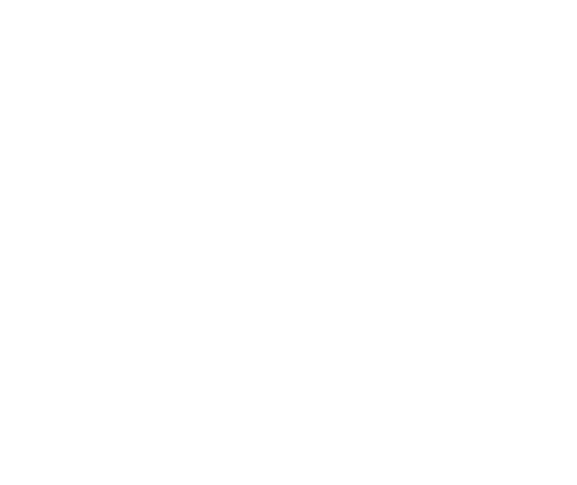
\includegraphics[width=\columnwidth]{./imagens/embranco.png}
    \renewcommand{\figurename}{Fig.}
    %\caption{Diagrama de Blocos do Sistema de Suspensão Ativa.}
	\label{embranco}
\end{figure}
\begin{figure}[H]
	\centering
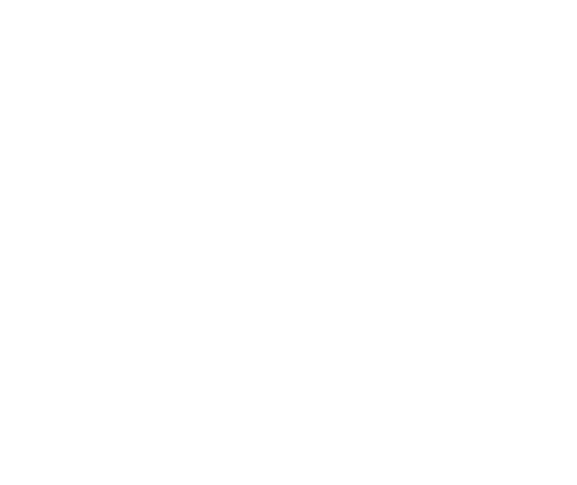
\includegraphics[width=.6\columnwidth]{./imagens/embranco.png}
    \renewcommand{\figurename}{Fig.}
    %\caption{Diagrama de Blocos do Sistema de Suspensão Ativa.}
	\label{embranco}
\end{figure}
\end{multicols}

\end{document}